\section{氨基酸}
\subsection{氨基酸的结构与分类}

根据氨基酸是否直接参与肽链合成,可分为蛋白质氨基酸和非蛋白质氨基酸;从营养价值来说,分为人体不能合成的必需氨基酸和人体能合成的非必需氨基酸。人体必需的氨基酸有:V、I、L、F、M、W、T、K、H,半必需氨基酸有R。其中,H曾被认为是半必需氨基酸。

\subsubsection{蛋白质氨基酸}

蛋白质氨基酸又称标准氨基酸,由遗传密码直接编码。在22种蛋白质氨基酸中,少见的是Sec和Pyl,它们也是最晚发现的两种蛋白质氨基酸。

Sec只存在于含硒蛋白中,如谷胱甘肽过氧化物酶和\ce{I3}去碘酶。克山病即由缺硒引起。

吡咯赖氨酸仅存在于部分产甲烷的古菌、某些G$^{+}$细菌(厚壁细菌、$\delta$-变形细菌)中。并且在产甲烷的古菌中,只有产甲烷的酶才含此氨基酸。

有时,进行氨基酸组成分析时,难以区分Asn/Asp和Gln/Glu,用Asx(B)和Glx(Z)代表。

下面列出了22种氨基酸的结构:(\autoref{fig:20种氨基酸}、\autoref{fig:pylsec})

\begin{figure}[htbp]
	\centering
	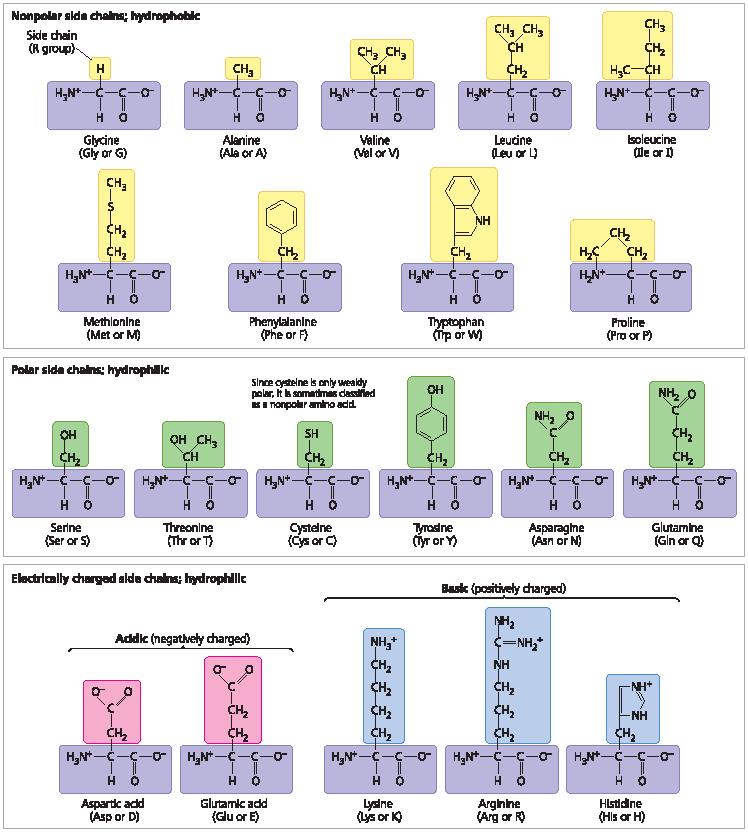
\includegraphics[width=\linewidth]{20种氨基酸.pdf}
	\caption{20种氨基酸}
	\label{fig:20种氨基酸}
\end{figure}

\begin{figure}[htbp]
	\centering
	\includegraphics[width=0.4\linewidth]{Pics/Pyl和Sec}
	\caption{硒代半胱氨酸和吡咯赖氨酸}
	\label{fig:pylsec}
\end{figure}


所有氨基酸都溶于水,只是溶解性不同。

\subsubsection{非蛋白质氨基酸}

非蛋白质氨基酸在合成时不会直接掺入肽链,具体分为下面两种情况:
\begin{enumerate}
	\item 翻译后经化学修饰,如胶原上的羟脯氨酸和羟赖氨酸;
	\item 从不参入蛋白质当中,如神经递质GABA、维生素泛酸的组分$\beta$-丙氨酸、尿素循环中的鸟氨酸、瓜氨酸。
\end{enumerate}

\subsection{氨基酸的性质和功能}

\subsubsection{氨基酸的共同性质}

\paragraph{缩合反应}

即一个氨基酸的氨基和另一个氨基酸的羧基发生缩合反应。

\paragraph{手性}

除了Gly,其他所有氨基酸都至少有一个不对称碳原子(Thr和Ile有两个),即手性碳原子。对于氨基酸手性的判断,在费歇尔投影式中,把羧基放上面、R基放下面,氢原子和氨基一左一右。氨基在左边,则是L-氨基酸;氨基在右边,则是D-氨基酸。

\begin{figure}[htbp]
	\centering
	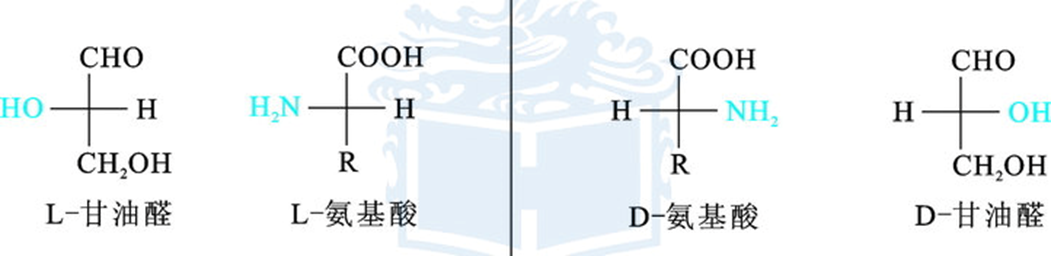
\includegraphics[width=0.8\linewidth]{Pics/L,D-aas}
	\caption{L型、D型氨基酸和甘油醛}
	\label{fig:ld-aas}
\end{figure}


核糖体合成时掺入的氨基酸都是L型。生物合成的蛋白质中,若有D-氨基酸,则一定是合成后异构酶催化的产物,如短杆菌肽、肽聚糖、羊毛硫抗生素、芋螺毒素。

具有手性的分子一般有旋光性,即对偏振光的振动方向产生旋转的特性。一对对映异构体的旋光方向正好相反。氨基酸的L或D型和旋光的方向没有必然联系,具体如何需要通过旋光仪测定。

\begin{gs}[:手性]
	\hspace{2em}在Lewis Carroll的童话世界里,爱丽丝对镜子里的“玻璃奶”充满了好奇,但现实中,这种奶可不好消化。为什么呢?因为生物体内只可以消化和吸收L型蛋白质、D型糖,“玻璃奶”的氨基酸和糖的手性相反,自然不能消化。

	\hspace{2em}制药工程师们现在特别关注药物的“手性”,因为不同的分子形态可能会带来完全不同的效果。比如,1960年欧洲的沙利度胺(thalidomide)事件,这种药物有两种形态,一种能镇静,另一种却会导致婴儿畸形。还有抗组胺药,一种让你昏昏欲睡,另一种则是减充血的好帮手。

	\hspace{2em}有趣的是,我们的味觉和嗅觉也分子的“手性”有关。比如,香芹酮(carvone)的两种构型,一种闻起来像薄荷,另一种则像橙子。柠檬烯(limonene)也是如此,一种闻起来像柠檬,另一种则像橙子。
\end{gs}

\paragraph{特殊酸碱性质与等电点}

氨基酸同时具有酸性的羧基和碱性的氨基,这使得它具有特殊的解离性质。氨基酸的酸性和碱性都弱于单独的胺或羧酸。氨基酸在生理情况下,主要是两性离子:由于其内部的酸碱反应,在一个分子上具有正负两种电荷。

氨基、羧基、有的氨基酸的R基在特定pH下可解离,影响着氨基酸的带电状态。使氨基酸不带电的pH值,称为该氨基酸的等电点。处在等电点的氨基酸,虽然也会少量解离,但解离出阴阳离子的数量相等。

可根据下面方法,在已知各基团的$\mathrm{p}K_{\text{a}}$情况下,计算氨基酸或短肽的等电点:
\begin{enumerate}
	\item 找出所有可解离基团,标注其$\mathrm{p}K_{\text{a}}$;
	\item 假定把该氨基酸(或短肽)放在极低pH下,此时所有基团都质子化;
	\item 逐步提高pH值,$\mathrm{p}K_{\text{a}}$越低的,越先放出质子;
	\item 写出所有可能的解离形式,并找出净电荷为零的那种;
	\item pI即为净电荷为零的情况时,两侧的$\mathrm{p}K_{\text{a}}$相加除以2。
\end{enumerate}

由此,可归纳:
\begin{itemize}
	\item 侧链无可解离基团的氨基酸,pI即两个$\mathrm{p}K_{\text{a}}$除以2;
	\item 酸性氨基酸,pI是两个较低的$\mathrm{p}K_{\text{a}}$除以2;
	\item 碱性氨基酸,pI是两个较高的$\mathrm{p}K_{\text{a}}$除以2.
\end{itemize}

\paragraph{R基团的疏水性}

氨基酸的疏水性直接影响蛋白质的折叠:
\begin{itemize}
	\item 疏水氨基酸一般位于蛋白质内部;
	\item 亲水氨基酸一般位于表面,但是带相反电荷的亲水氨基酸也可以成对出现在蛋白质内部。
\end{itemize}

\paragraph{氨基酸的氨基和羧基参与的化学反应}

\subparagraph{与2,4-二硝基氟苯(DNFB)}

\begin{itemize}
	\item 反应基团:$\alpha$-氨基;
	\item 反应条件:弱碱性;
	\item 产物:黄色的DNP-氨基酸,Pro也可以;
\end{itemize}

肽也可以与DNFB反应,生成DNP-肽。用酸水解后可得到肽链N端氨基酸形成的DNP-氨基酸,再用有机溶剂萃取,可鉴定肽链的N端氨基酸。这叫做蛋白质的Sanger测序。

\subparagraph{与异硫氰酸苯酯(PITC)}

\begin{itemize}
	\item 反应基团:$\alpha$-氨基;
	\item 反应条件:弱碱性;
	\item 产物:PTC-氨基酸$\xrightarrow{\text{酸性}}$PTH-氨基酸,Pro也可以;
\end{itemize}

若是肽与PITC反应,会先生成PTC-肽。之后调节pH至酸性,可释放出N端的PTH-氨基酸。用乙酸乙酯可抽提出PTH-氨基酸。由此,可设计出从N端进行肽链测序的方法,称为Edman降解法。

\subparagraph{与茚三酮}

\begin{itemize}
	\item 反应基团:整个氨基酸;
	\item 反应条件:加热,弱酸性;
	\item 产物:蓝紫色物质(可在\SI{570}{\nm}处比色),Pro生成黄色物质;
\end{itemize}

该反应非常灵敏,常用于法医采集指纹。

氨基酸与其他物质发生的反应归纳在\autoref{tab:aminoAcidInvolvedReactions}中。

\begin{table}[htbp]
	\zihao{5}
	\centering
	\begin{NiceTabularX}{\textwidth}{>{\centering\arraybackslash}m{4em}>{\centering\arraybackslash}m{6em}>{\centering\arraybackslash}m{12em}X}[hvlines]
		\textbf{反应类型} & \textbf{反应试剂} & \textbf{主要反应产物} & \Block[c]{1-1}{\textbf{用途}} \\
		\Block[v-center]{6-1}{$\alpha$-氨基} & 亚硝酸 & 羟酸,\ce{N2} & Van Slyke 定氮 \\
		& 甲醛 & 二羟甲基氨基酸 & 氨基酸滴定 \\
		& 酰化试剂:苄氧酰氯、叔丁氧酰氯、对甲苯磺酰氯、丹磺酰氯等 & 酰化氨基酸 & \Block[l]{1-1}{肽的人工合成氨基的保护;丹磺酰氯可用于N-端氨基酸的标记和微量氨基酸的定量} \\
		& DNFB & DNP-氨基酸 & \Block[l]{2-1}{多肽和蛋白质N-端氨基酸的鉴定} \\
		& PITC & PTC氨基酸,PTH氨基酸 &  \\
		& 氨基酸氧化酶、转氨酶等 & 酮酸等 & 细胞内氨基酸的代谢 \\
		\Block[v-center]{2-1}{$\alpha$-羧基} & 碱 & 氨基酸盐 & \Block[l]{2-1}{氨基酸羧基的保护和活化} \\
		& 醇 & 氨基酸酯 &  \\
		\Block[v-center]{4-1}{$\alpha$-氨基和$\alpha$-羧基} & tRNA、氨酰-tRNA合成酶、ATP等 & 氨酰-tRNA & 蛋白质的生物合成 \\
		& 脱羧酶 & 胺 & 氨基酸的代谢 \\
		& 茚三酮 & 紫色物质,Pro为黄色物质 & 氨基酸的定性和定量 \\
		& 肽酰转移酶等 & 肽 & 多肽和蛋白质的生物合成
	\end{NiceTabularX}
	\caption{氨基酸参与的反应}
	\label{tab:aminoAcidInvolvedReactions}
\end{table}

\subsubsection{个别氨基酸的特殊性质}

\paragraph{F、Y、W的紫外吸收性质}

Phe、Tyr、Trp三种氨基酸的侧链含有苯环,赋予它们近紫外吸收的效应。Trp的紫外吸收最强。Tyr与Trp的吸收峰都靠近\SI{208}{\nm}。

\paragraph{亲水和疏水基团}

疏水基团缺乏反应性,多数时候起到驱动蛋白质折叠的作用,少数蛋白质利用疏水侧链形成口袋结合脂溶性物质。

亲水氨基酸的侧链具有反应性,参与行使多种生物学功能。
\begin{description}
	\item[羟基] S、T、Y三种氨基酸侧链具有羟基,可被磷酸化修饰。
	\item[$\epsilon$-氨基] K具有$\epsilon$-氨基,可作为亲和基团参与酶的催化,与羧基形成酰胺键实现共价连接,与醛基形成席夫碱,发生乙酰化、甲基化、泛酰化修饰。
	\item[巯基和硒醇基] C的巯基可作为亲核基团参与催化。两个巯基可被氧化形成二硫键。U含有还原性更强的硒醇基,具有抗氧化活性。
	\item[咪唑基] H的咪唑基,$\mathrm{p}K_{\text{a}}$约为7,使得它在生理条件下可以作为质子的供体和受体。许多酶的活性中心含有H。咪唑基也可以发生磷酸化修饰。
	\item[羧基] Asp和Glu侧链上含有羧基,在特定情况下可以作为质子的供体和受体,参与广义酸碱催化。羧基带负电荷的特性也可结合金属离子。
\end{description}

\subsection{氨基酸的功能}

\begin{itemize}
	\item 形成肽;
	\item 多种生物活性物质的前体;
	\item 作为神经递质;
	\item 碳骨架氧化分解产生ATP;
	\item 碳骨架作为糖异生或酮体合成的原料。
\end{itemize}

\section{蛋白质的结构}

\subsection{肽}

\subsubsection{肽的分类}
肽即是氨基酸之间发生缩合,形成酰胺键(肽键)产生的聚合物。一般把50个氨基酸残基以上的肽称为蛋白质,因此,具有51个氨基酸残基的胰岛素就是最小的蛋白质。截至\today,最大的蛋白质是PKZILLA-1,来自小定鞭金藻(\textit{Prymnesium parvum})。在此之前,最大的蛋白质被认为是肌巨蛋白。

\subsubsection{肽的理化性质}

\begin{description}
	\item[旋光性] 一种寡肽只要不是全由Gly构成,它就具有旋光性。
	\item[两性解离] 解离基团较少的肽,滴定曲线和单个氨基酸相似。只有小肽才可以使用前述的方法计算pI。
	\item[双缩脲反应] 高中讲过。至少两个肽键(三肽)才可发生此反应。
	\item[水解反应] 肽键可在特定条件水解。
\end{description}

\subsubsection{几种天然活性肽}

活性肽可分为两类:在核糖体上合成的、不在核糖体上合成的。(\autoref{tab:commonBioactivePeptides})
\begin{itemize}
	\item 在核糖体上合成的:只会引入L-氨基酸,形成的肽键总是$\alpha$-氨基与$\alpha$-羧基构成的。通常合成的是前体,经过切割才得到活性肽。
	\item 不在核糖体上合成的:这类肽在不由基因组直接编码,而是通过酶催化合成。它可能含有D-氨基酸,也可能不是严格由是$\alpha$-氨基与$\alpha$-羧基形成肽键(如谷胱甘肽的第一个肽键)。
\end{itemize}

\begin{table}[htbp]
	\centering
	\begin{NiceTabularX}{\textwidth}{>{\centering\arraybackslash}m{5em}cc>{\centering\arraybackslash}m{8em}C}[hvlines]
		类型和种类 & 来源 & 类别 & 功能 & 备注 \\
		\Block{1-5}{非核糖体合成肽} &  &  &  &  \\
		\Block[v-center]{1-1}{谷胱甘肽} & \Block[v-center]{1-1}{动植物细胞} & \Block[v-center]{1-1}{三肽} & \Block[v-center]{1-1}{抗氧化} & 第一个肽键为$\gamma$-肽键 \\
		短杆菌肽 S & 细菌 & 环十肽 & 抗菌 & 含有 D-氨基酸 \\
		肽聚糖中寡肽 & 细菌细胞壁 & 小肽 & 形成细菌细胞壁的网络结构 & 含有 D-氨基酸 \\
		肌肽 & 肌肉细胞 & 二肽 & 不明 & 含有$\beta$-丙氨酸 \\
		\Block{1-5}{核糖体合成多肽} &  &  &  &  \\
		\Block[v-center]{1-1}{TRH} & \Block[v-center]{1-1}{下丘脑} & \Block[v-center]{1-1}{三肽} & \Block[v-center]{1-1}{促甲状腺素释放} & N端焦谷氨酰化,C端酰胺化 \\
		OT & 垂体后叶 & 八肽 & 刺激子宫收缩、排乳、促遗忘 &  \\
		ADH & 垂体后叶 & 八肽 & 升血压、抗利尿、促记忆 &  \\
		$\alpha$-鹅膏蕈碱 & 鬼笔鹅蕈类真菌 & 环八肽 & 真核RNA pol II 强抑制剂 &
	\end{NiceTabularX}
	\caption{常见的生物活性肽}
	\label{tab:commonBioactivePeptides}
\end{table}

\subsection{蛋白质的结构}

蛋白质结构的四个层次是:一级结构、二级结构、三级结构、四级结构。并不是所有蛋白质都含有三级和四级结构。

\subsubsection{蛋白质的一级结构}

蛋白质的一级结构就是氨基酸的排列顺序、二硫键的数目和位置。

肽键具有下面性质:
\begin{description}
	\item[部分双键的性质] 键长介于\ce{C=N}和\ce{C-N}之间。肽键具有的部分双键性质是酰胺N上的孤对电子与相邻羰基C发生共振的结果。
	\item[多为反式(\textit{trans}),也有顺式(\textit{cis})] 核糖体上形成的肽键均为反式。由于空间位阻,反式构象比顺势构象稳定100倍。若出现X-Pro,则由于Pro的四氢吡咯环空间位阻非常大,几乎抵消了反式构象的优势,只比顺式稳定4倍,故此时肽键可以存在顺式构象。蛋白质合成好后,与Pro的亚氨基有关的肽键可被肽基脯氨酰顺反异构酶(PPI)催化变为顺式。
	\item[与肽键有关的6个原子共平面] 该平面称为肽平面或酰胺平面。共面性质是肽键不可旋转带来的。由\autoref{fig:peptidePlane}可见,两个肽平面以C$_{\alpha}$相关,且是两个可自由旋转的单键。规定:\ce{C_{\alpha}-N}旋转形成的为$\phi$角,\ce{C_{\alpha}-C}旋转形成的为$\psi$角。与同一个C$_{\alpha}$相关的$\phi$和$\psi$角称蛋白质的二面角。

	\begin{figure}[htbp]
		\centering
		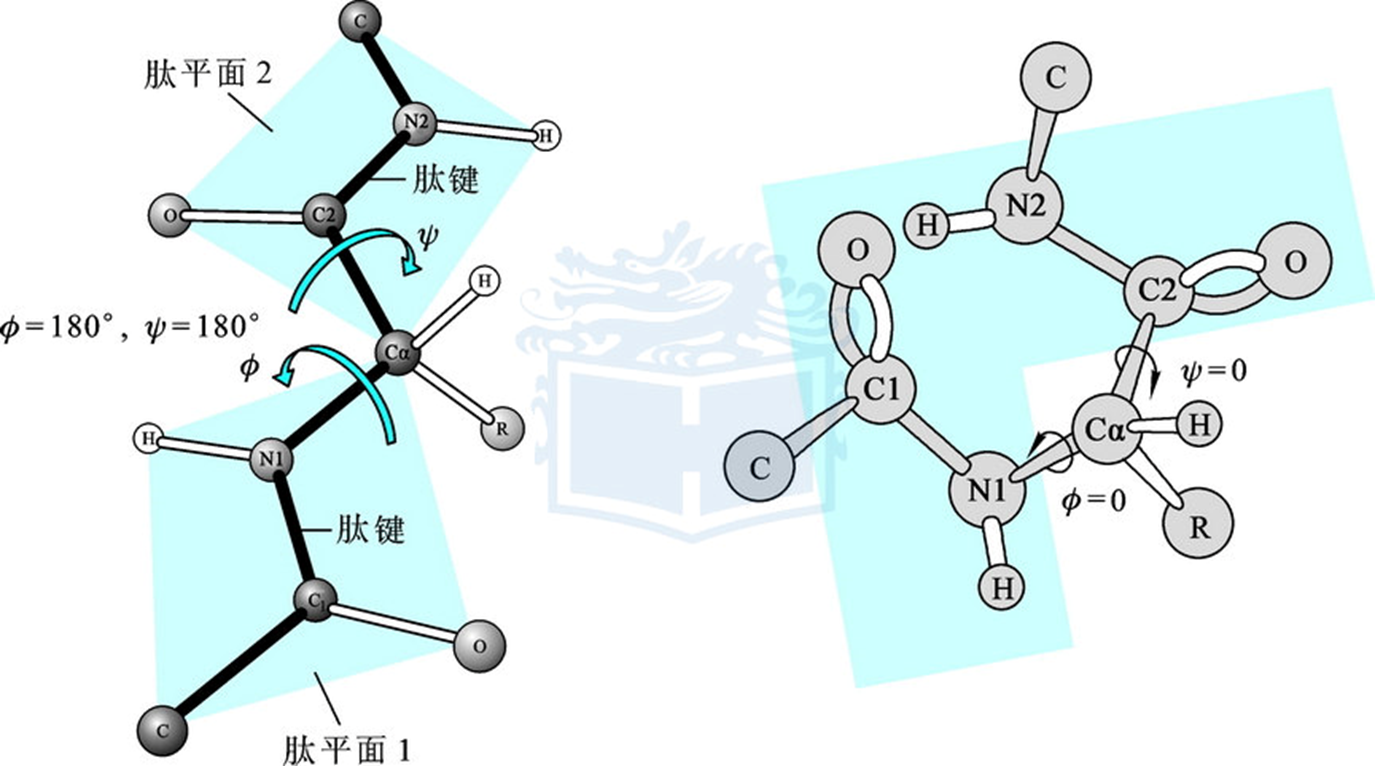
\includegraphics[width=0.8\linewidth]{Pics/肽平面}
		\caption{肽平面和二面角}
		\label{fig:peptidePlane}
	\end{figure}

	二面角的大小是这样规定的:
	\begin{itemize}
		\item 所有肽键共面时,$\psi$和$\phi$角定为$\pm$\SI{180}{\degree};
		\item 若$\psi$的旋转单键\ce{C_{\alpha}-C}两侧的两条化学键呈顺式,则$\psi=0$,$\phi$角同理;
		\item 以\ce{C_{\alpha}}向碳原子和氮原子看,单键顺时针旋转则为正值、逆时针旋转则为负值。
	\end{itemize}

	\begin{qj}[:谁是$\psi$角、谁是$\phi$角?]
		\ce{C_{\alpha}-C}旋转形成的为$\psi$角,可以用$\psi$的形状像横着的C加一竖来联想。
		\ce{C_{\alpha}-N}含氮,“蛋(氮)”是圆的,也就是$\phi$的圆圈。
	\end{qj}

	\begin{tx}[:此二面角非彼二面角]
		这里的二面角和数学立体几何的二面角没有任何关系。此二面角并非两个肽平面的夹角。
	\end{tx}

	在Ramachandran图(\autoref{fig:ramachandran})中,所有可能二面角以坐标$(\phi,\psi)$对应的点表示,形成了图中的有色区域。由于侧链基团的限制,二面角并不能自由变化。

	\begin{figure}[htbp]
		\centering
		\includegraphics[width=0.4\linewidth]{Pics/Ramachandran图}
		\caption{Ramachandran图}
		\label{fig:ramachandran}
	\end{figure}

	\item[部分带电性] 酰胺N带部分正电荷,羰基O带部分负电荷。这是由于二者共振形成的。
\end{description}

\mbox{}

测定蛋白质一级结构的意义:
\begin{itemize}
	\item 有助于理解其三维结构和功能。蛋白质的一级结构包含了决定三维结构的全部信息。
	\item 在分子水平研究生物进化。
\end{itemize}

蛋白质一级结构数据库有:\href{https://cn.expasy.org}{PIR(Protein Information Resource)}、\href{https://www-nbrf.geogetown.edu}{SWISS-PROT}等。
\begin{description}
	\item[PIR] 包含从EMBL翻译来的蛋白质序列,经过检验和注释;
	\item[SWISS-PROT] 包含NCBI从GenBank翻译来的蛋白质序列。
\end{description}

\subsubsection{蛋白质的二级结构}

二级结构指的是肽链主链(不含R基)在局部形成的有规律的折叠和盘绕。二级结构稳定性主要由氢键决定。

常见的二级结构包括:$\alpha$螺旋、三股螺旋、$\beta$折叠、$\beta$转角、$\beta$凸起、无规卷曲和环。按照上述顺序,结构稳定性递减,但功能性递增,因为许多酶的活性中心都是无规卷曲和环构成。

\paragraph{$\alpha$螺旋}

该螺旋的主要特征:
\begin{itemize}
	\item 螺旋的形成是自发的。稳定螺旋的氢键很有规律:若第$n$位的氨基酸残基羰基O为氢键受体,则$n+4$位的氨基酸残基的氨基上H便是氢键供体。(\autoref{fig:hydrogenBondDonorsAndAcceptorsInVariousHelices})

	\begin{figure}[htbp]
		\centering
		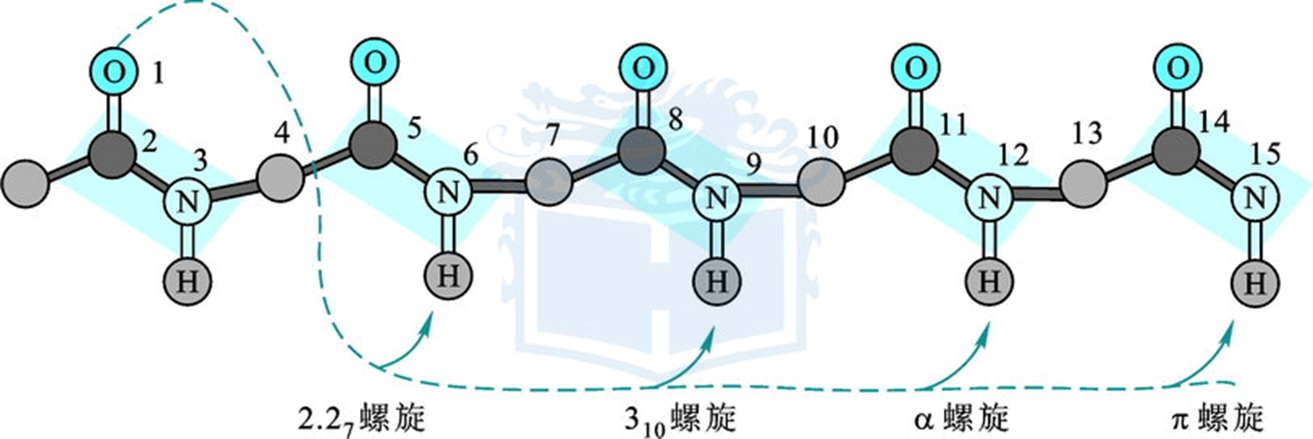
\includegraphics[width=0.8\linewidth]{Pics/各种螺旋的氢键供体与受体}
		\caption{各种螺旋的氢键供体与受体}
		\label{fig:hydrogenBondDonorsAndAcceptorsInVariousHelices}
	\end{figure}

	\item 每个3.6个残基,螺旋上升一圈。一个氨基酸残基环绕螺旋轴\SI{100}{\degree},螺距\SI{0.54}{\nm}。螺旋半径\SI{0.23}{\nm}。
	\item 螺旋方向一般是右手,因为L型氨基酸形成右手螺旋空间位阻小。
	\item 氨基酸残基的R基伸出在螺旋外表面,影响螺旋的形成的带电性。
\end{itemize}

使用多聚氨基酸来研究R基团对$\alpha$螺旋稳定性的影响。
\begin{itemize}
	\item 多聚Leu、多聚Ala容易形成;
	\item 多聚Gly只会形成无规卷曲,多聚Pro只会形成特有的右手螺旋或左手螺旋。
	\item 酸性和碱性氨基酸只有在不带电荷的pH值下才会形成。
\end{itemize}

一般而言,判断一个氨基酸残基是否有利于形成$\alpha$螺旋,要看其R基能否保护主链上的氢键。
\begin{itemize}
	\item Gly不利于形成$\alpha$螺旋,因为侧链太小,二面角变化太大;
	\item Pro通常比较少出现,因为其亚氨基无法作为氢键供体。它只可出现在$\alpha$螺旋的前四个残基中,因为前四个残基不承担氢键供体的角色,如在视紫红质中GPCR;
	\item Ile、Val、Thr、Phe、Trp因为侧链比较大,有较大空间位阻;
	\item Ser、Asp、Asn侧链在靠近主链的位置有氢键供体或受体,可竞争主链的氢键;
	\item 侧链带电荷(没有His),若是同种电荷连续排列,也不利于$\alpha$螺旋形成。
\end{itemize}

偶极矩也是影响$\alpha$螺旋稳定性的因素。螺旋具有一个总偶极矩,正极在N端,负极在C端。螺旋可借助N端的酸性氨基酸和C端的碱性氨基酸来中和偶极矩,或者通过与带电荷的基团或金属离子结合来中和。

用螺旋轮作图可显示出各个氨基酸残基在螺旋边缘的分布情况,有利于判断一个螺旋的亲、疏水性。疏水$\alpha$螺旋经常出现在膜内在蛋白的跨膜区,

\begin{itemize}
	\item 若螺旋上亲水氨基酸较多,则为亲水$\alpha$螺旋;
	\item 若疏水氨基酸较多,则为疏水$\alpha$螺旋,常常出现在膜内在蛋白的跨膜区,如GPCR;
	\item 若二者差不多多,并且亲水氨基酸和疏水氨基酸各分布在螺旋的一侧,则是两亲$\alpha$螺旋,
\end{itemize}

除此$\upalpha$螺旋之外,Pauling还提出了其他螺旋:

\begin{table}[htbp]
	\centering
	\begin{tabularx}{\textwidth}{|c|c|c|C|}
		\hline
		螺旋类型 & 每圈氨基酸残基数 & 氢键环原子数 & 氢键供体位置 \\ \hline
		$2.2_{7}$螺旋 & 2.2 & 7 & $n+2$位残基的氨基H \\ \hline
		$3_{10}$螺旋 & 3 & 10 & $n+3$位残基的氨基H \\ \hline
		$4.4_{16}$螺旋 & 4.4 & 16 & $n+5$位残基的氨基H \\ \hline
	\end{tabularx}
	\caption{其他螺旋}
	\label{tab:many_helix}
\end{table}

在蛋白质中,主要都是$\alpha$螺旋,还没有发现$2.2_{7}$螺旋。

\paragraph{$\beta$折叠}

\paragraph{$\beta$转角}

\paragraph{$\beta$凸起}

\paragraph{无规卷曲与环}

\subsubsection{蛋白质的三级结构}

三级结构可以说就是单条肽链所形成的完整三维结构。三级结构通常由模体和结构域两种超二级结构组成。一种蛋白质的全部三维结构称为构象。

\begin{tx}[:区分“构象”与“构型”]
	构型是指在立体异构中,特定的原子和基团在空间上的几何布局。构型变化必然伴随共价键的断裂和重新形成。构象的转变就只是单键自由旋转造成的。
\end{tx}

\paragraph{稳定三级结构的化学键}

这些化学键主要是次级键,包括:氢键、疏水键、离子键、范德华力。此外,金属配位键、二硫键也发挥一定作用。

\begin{description}
	\item[氢键] 与电负性强的原子相连的氢原子,带部分正电荷,可作氢键供体;一些电负性较强,带部分负电荷的原子则作为氢键受体。在三级结构中,氢键的供体、受体主要来源于氨基酸侧链基团,而不是二级结构里,来自主链。
	\item[离子键] 即静电作用。又称为盐键、盐桥。离子键的形成主要依赖于带电荷的氨基酸侧链基团和肽链首尾游离的氨基、羧基。
	\item[疏水键] 疏水基团或疏水分子在水溶液里为了避开水相互聚集的作用力就是疏水键(疏水作用力)。主要由疏水氨基酸残基提供。疏水氨基酸会在蛋白质内部形成疏水核心。疏水键是稳定三级结构最重要的作用。
	\item[范德华力]
	\item[配位键] 配位键对某些金属蛋白的稳定起作用。
	\item[二硫键] 含有二硫键的蛋白质一般是分泌蛋白或膜蛋白,胞内蛋白很少有二硫键。但是古菌很多胞内蛋白质也具有二硫键。
\end{description}

\paragraph{三级结构的部件}

\subparagraph{模体}

模体的概念有两个,一个指的是一级结构,即氨基酸的特定序列(序列模体)。另一个介于三级结构和二级结构之间,即结构模体。

结构模体是由相邻的二级结构单位的疏水氨基酸残基相互作用,形成的二级结构组合体。

常见的模体有:

%\begin{table}[]
%	\centering
%	\begin{tabularx}{\textwidth}{|c|m{10em}|l|X|}
%		\hline
%		\textbf{模体} & \multicolumn{1}{c|}{\textbf{结构特点}} & \multicolumn{1}{c|}{\textbf{功能}} & \multicolumn{1}{c|}{\textbf{存在}} \\ \hline
%		卷曲螺旋 & 多股$\alpha$螺旋聚合体形成左手超螺旋,螺旋之间平行或反平行,含七肽重复序列 & 蛋白质折叠、相互作用 & SNARE \\ \hline
%		HLH & 两个螺旋、中间一个环 & 环用来结合\ce{Ca^{2+}},碱性HLH这类模体可结合DNA大沟 & 传感器蛋白、转录因子 \\ \hline
%		$\beta$-$\alpha$-$\beta$ & 平行的$\beta$折叠、$\alpha$螺旋 &  &  \\ \hline
%		$\beta$发夹环 & 两股反平行$\beta$股和一段连接小环 &  &  \\ \hline
%		HTH & 如图 & 一个alpha螺旋以亲水氨基酸残基结合DNA & 与DNA特异结合的蛋白质 \\ \hline
%		Rossmann折叠 & 形成$\beta$  含有疏水核心 &  & 需要辅酶I或辅酶II的酶 \\ \hline
%		希腊钥匙 & 全$\beta$折叠聚合体 &  & 清蛋白原、质体蓝素 \\ \hline
%		$\beta$螺旋 & 多个$\beta$股,右手或左手 & 促进蛋白质相互作用 & 果胶酸裂合酶(右手) \\ \hline
%	\end{tabularx}
%	\caption{蛋白质结构模体}
%	\label{tab:structure_motif}
%\end{table}

\subparagraph{结构域}

较大的蛋白质一般会折叠成多个相互独立的球状区域,即结构域。疏水核心是结构域稳定存在必需的。结构域有大有小,但不会太大。大的结构域疏水核心较大,更稳定;小的结构域疏水核心较小,不稳定,需要靠金属离子或二硫键加固。

结构域在结构和功能上都是独立的。许多蛋白质的结构域被人为分开后,依然能保持活性。

\subsubsection{蛋白质的四级结构}


\subsection{蛋白质的折叠历程}

\section{蛋白质结构和功能之间的关系}

\subsection{蛋白质的功能}

\subsection{蛋白质结构和功能之间的关系}

\subsection{几种重要的蛋白质和功能}

\subsubsection{纤维状蛋白质}

\paragraph{$\alpha$角蛋白}

\paragraph{$\beta$角蛋白}

\paragraph{胶原蛋白}

\subsubsection{球状蛋白——珠蛋白}

\subsubsection{球状蛋白——免疫球蛋白}

\subsubsection{膜蛋白}

\subsubsection{天然无折叠蛋白}


\section{核苷酸}

\subsection{核苷酸的结构与组成}

$\text{核苷酸}=\text{核苷}+\text{磷酸基团}=\text{D-核糖或D-脱氧核糖}+\text{碱基}+\text{磷酸基团}$,碱基和戊糖之间通过$\beta$-N-糖苷键连接。

\subsubsection{碱基}

碱基即含氮碱基,包括嘌呤和嘧啶。它们的结构及原子编号见\autoref{fig:puring_pyrding}。

嘧啶为六元芳香杂环,平面结构;嘌呤由六元的嘧啶环和五元的咪唑环融合而成,实验表明两个环之间成一定角度,尽管理论上应当是平面结构。

常见的碱基有腺嘌呤(A)、鸟嘌呤(G)、胞嘧啶(C)、胸腺嘧啶(T)、尿嘧啶(U)五种。RNA与DNA共有的是A、G、C,而U通常只存在于RNA,T通常只存在于DNA,不过也有例外。如tRNA上的T$\upPsi$C环中含有T碱基,有时DNA上会出现U。
\begin{figure}
	\centering
	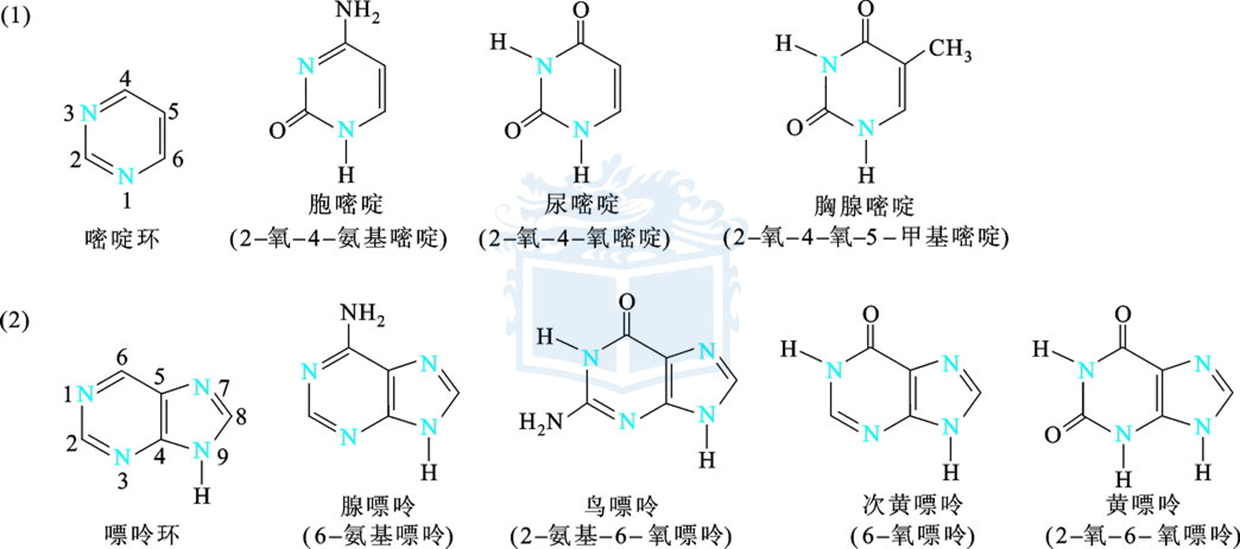
\includegraphics[width=\linewidth]{Pics/嘧啶环和嘌呤环的编号以及各种碱基的化学结构}
	\caption{嘧啶环和嘌呤环的编号以及各种碱基的化学结构}
	\label{fig:puring_pyrding}
\end{figure}


机体的修饰碱基有:5-甲基胞嘧啶(m$^{5}$C)、N$^{6}$-甲基腺嘌呤(m$^{6}$A)、黄嘌呤(X)、次黄嘌呤(I)等。m$^{5}$C和m$^{6}$A具有表观遗传功能,可抑制所在基因的表达,其中线虫、果蝇基因组中含有的是m$^{6}$A。

茶碱和咖啡因是腺苷(A)的类似物,可以与肌细胞和脑细胞膜上的腺苷受体结合,提高心率和产生兴奋,这便是喝茶或咖啡提神的原理;还可以在胞内充当催化cAMP水解的磷酸二酯酶的抑制剂,加强依赖cAMP通路的激素的作用效果。

碱基具有以下化学性质:
\begin{description}
	\item[紫外吸收] 碱基的共轭双键赋予其紫外吸收性质,最大吸收值在\SI{260}{\nano\meter}。
	\item[可发生互变异构] 嘧啶碱基:酮式$\rightleftharpoons$烯醇式,腺嘌呤:氨基式$\rightleftharpoons$亚氨基式。这两种互变异构体在体内都以前者为极多,但是碱性条件下可向后者移动。碱基互补配对规则只适用于酮式和氨基式的碱基。(\autoref{fig:base_change})

	\begin{figure}[htbp]
		\centering
		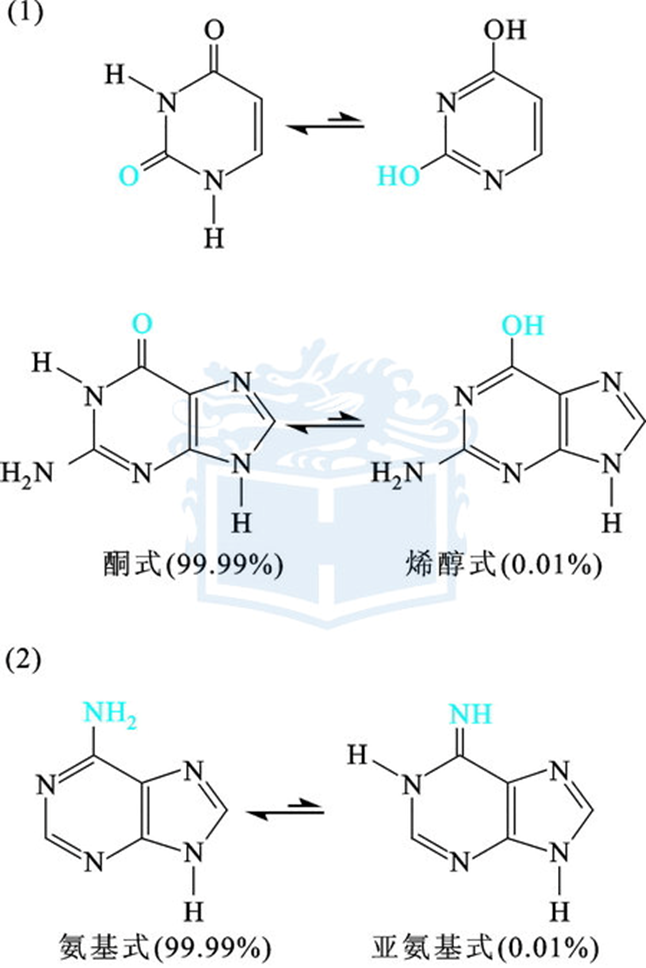
\includegraphics[width=0.5\linewidth]{Pics/碱基互变异构}
		\caption{碱基互变异构}
		\label{fig:base_change}
	\end{figure}

	\item[水溶性差] 这是由碱基的芳香杂环决定的。因此能形成稳定的DNA双螺旋结构。
	\item[解离] pH决定了环上各个N原子是否与\ce{H+}结合,影响氢键的供受体关系、碱基配对规则。中性条件下,碱基主要以内酰胺形式存在。
\end{description}

\subsubsection{核苷}

核苷是碱基和核糖通过$\beta$-N-糖苷键形成的糖苷。该糖苷键由核糖的异头C与嘧啶碱基的N1或嘌呤碱基的N9形成。(\autoref{fig:structure_nucleoside})

\begin{figure}[htbp]
	\centering
	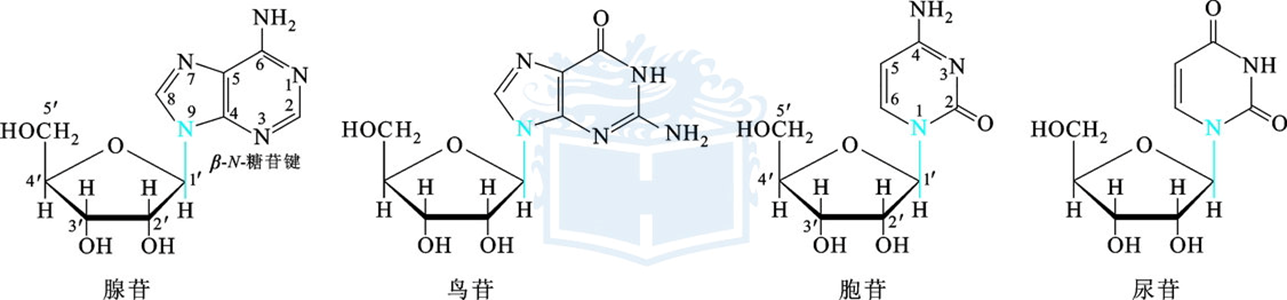
\includegraphics[width=\linewidth]{Pics/核苷的结构}
	\caption{核苷的结构}
	\label{fig:structure_nucleoside}
\end{figure}

生物体内核苷的糖苷键都是$\beta$-N-糖苷键,$\beta$的意思是碱基在核糖环上方。生物体内的核苷没有$\alpha$-N-糖苷键。

嘧啶核苷只有反式构象,嘌呤核苷多数是反式构象,仅在Z-DNA中是顺式。(\autoref{fig:syn_anti_nucleoside})

\begin{figure}[htbp]
	\centering
	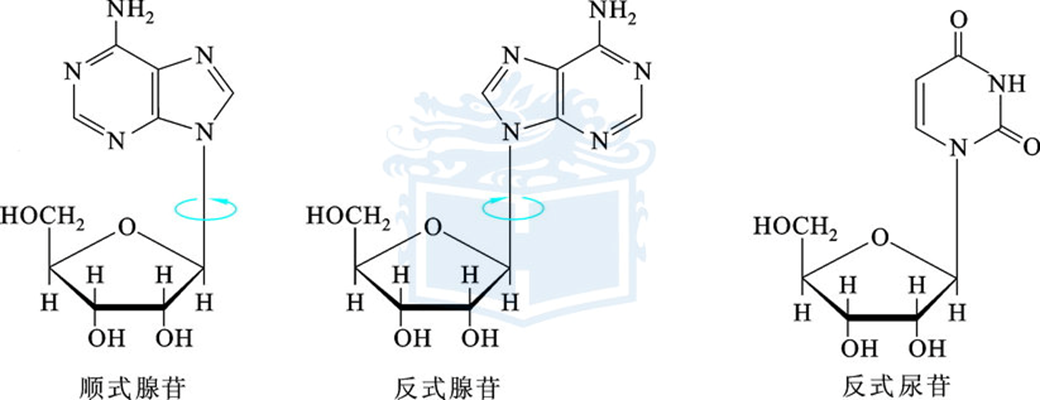
\includegraphics[width=0.7\linewidth]{Pics/核苷的构象}
	\caption{核苷的构象}
	\label{fig:syn_anti_nucleoside}
\end{figure}

常见的核苷如\autoref{fig:structure_nucleoside}所示。它们的核糖变为脱氧核糖,就是脱氧核苷。

修饰核苷是指碱基有修饰的、或核糖有修饰的、或以特殊成键方式存在的核苷。例如假尿苷($\upPsi$),是以C5与核糖相连。(\autoref{fig:modified_nucleoside})

\begin{figure}[htbp]
	\centering
	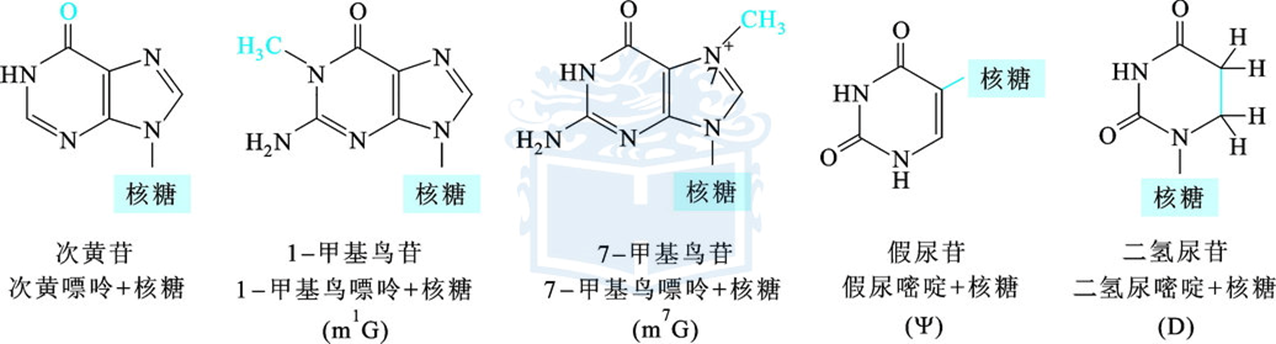
\includegraphics[width=\linewidth]{Pics/几种修饰核苷}
	\caption{几种修饰核苷}
	\label{fig:modified_nucleoside}
\end{figure}

核苷的性质如下:

\begin{description}
	\item[水溶性] 因为核糖亲水,所以核苷的水溶性比单独的碱基高。
	\item[水解] 只有嘌呤核苷容易被酸水解,意思是:所有核苷可抵抗碱水解、嘧啶核苷还可抵抗酸水解。
\end{description}

\subsubsection{核苷酸}

自然界的核苷酸多为核苷-5′-磷酸。(\autoref{fig:structuresOfCommonNucleotides})

\begin{figure}[htbp]
	\centering
	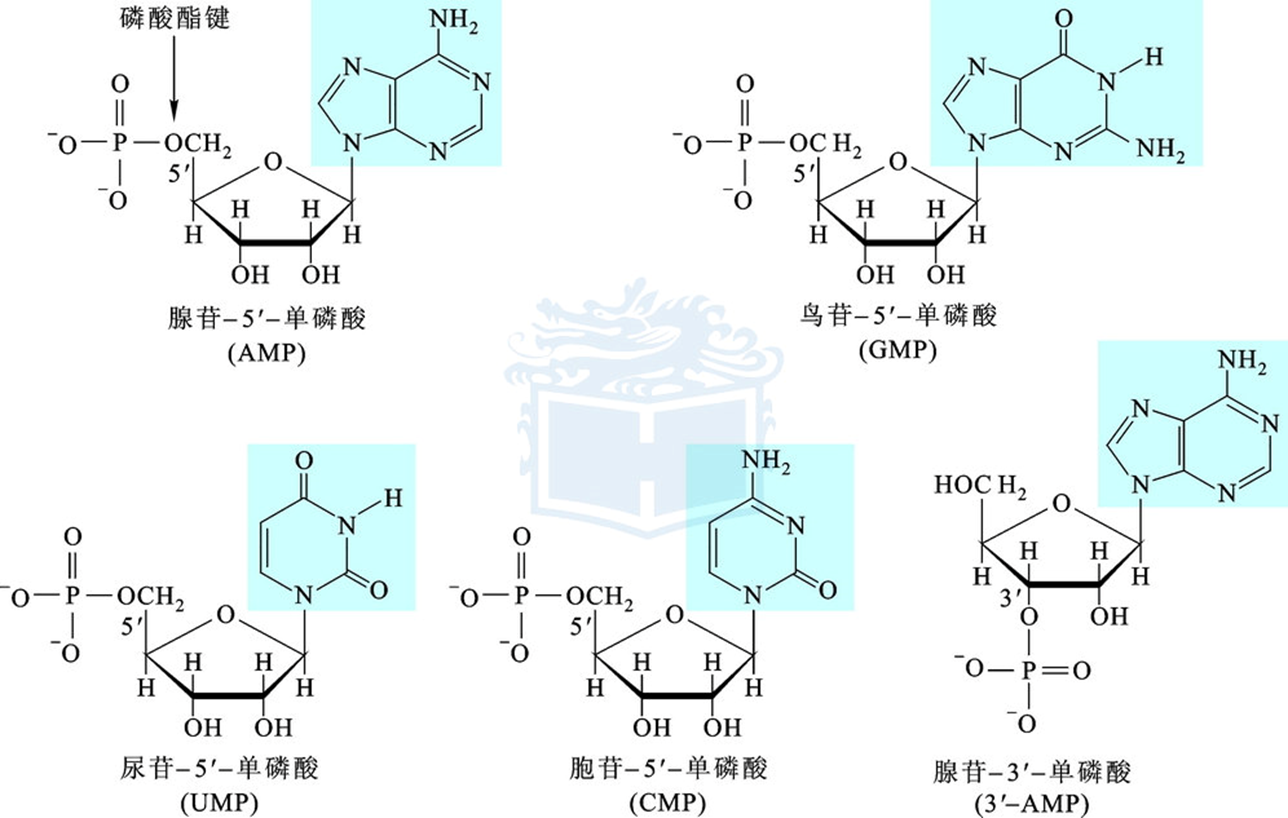
\includegraphics[width=0.9\linewidth]{Pics/常见核苷酸的结构}
	\caption{常见核苷酸的结构}
	\label{fig:structuresOfCommonNucleotides}
\end{figure}

核苷酸的磷酸基团还可以增加到3个。这三个磷酸基团从最靠近核糖的那个开始,依次称为$\alpha$、$\beta$、$\gamma$磷酸。

某些核苷三磷酸可形成环核苷酸,作为第二信使。

核苷酸的构象不是固定不变的,而是具有一定柔性。

核苷酸的理化性质由组成它的核糖、碱基等决定。

\section{核酸的结构与功能}

\subsection{核酸的分类}

核酸分为核糖核酸(RNA)和脱氧核糖核酸(DNA),二者直接的区别就是构成它们的戊糖,在2′位的是羟基还是氢原子。

因为RNA有2′-OH,所以理论上可以形成2′-5′磷酸二酯键。只有在高等动物体内干扰素在作用时才诱导靶细胞合成以2′-5′磷酸二酯键相连接的多聚A。

DNA和RNA的差别列在\autoref{tab:DNA_RNA}中:

\begin{table}[htbp]
	\centering
	\begin{tabularx}{\textwidth}{|c|C|C|}
		\hline
		\textbf{性质} & \textbf{RNA} & \textbf{DNA} \\ \hline
		戊糖 & D-核糖 & 2′-D-脱氧核糖 \\ \hline
		碱基 & 第四个碱基通常是U & 第四个碱基通常是T \\ \hline
		多聚核苷酸链的数目 & 多为单链 & 多为双链 \\ \hline
		在细胞内的双螺旋 & A型 & B型和Z型 \\ \hline
		种类 & 多种 & 只有一种 \\ \hline
		功能 & 功能多样 & 仅充当遗传物质 \\ \hline
		碱溶液下的稳定性 & 不稳定,很容易水解 & 稳定 \\ \hline
	\end{tabularx}
	\caption{DNA和RNA的比较}
	\label{tab:DNA_RNA}
\end{table}

DNA和RNA主要有三点差别:
\begin{description}
	\item[戊糖:RNA是核糖,DNA是脱氧核糖] 这是判断核酸是DNA还是RNA的唯一标准。RNA的2′-OH是具有反应性的亲核基团,使之容易碱水解。不易降解的RNA,如rRNA和tRNA,其上很多2′-OH都被甲基化,失去反应性。
	\item[碱基:RNA是U,DNA是T] DNA上正常无U,相当于是标记上突变的碱基,便于修复。这项差别并不绝对。RNA中可能出现的T来自于U甲基化,DNA中的U来自于dUTP的错误掺入或C自发脱氨基。DNA天然含U的情形:
	\begin{itemize}
		\item 枯草杆菌PBS2噬菌体完全用U取代了基因组里的T;
		\item 昆虫化蛹时,调控酶的活性,掺入大量U进入DNA,作为细胞死亡的信号。
	\end{itemize}
	\item[单双链:RNA单链,DNA双链]DNA双链更稳定,RNA单链变化更多。但也不绝对。如一些病毒具有单链DNA或双链RNA。miRNA也是双链RNA。
\end{description}

生物体内有多种天然小RNA,功能多样。

\mbox{}

核酸具有一级结构、二级结构、三级结构,但没有四级结构。

\subsection{核酸的一级结构}

核酸的一级结构就是核苷酸或碱基的排列顺序。

核酸具有极性,单链的一头有游离的3′-OH,另一头有游离的5′-OH。

除了线型核酸外,在细菌、质粒、叶绿体、大多数线粒体DNA都是环形的。它们完全没有游离的3′-OH或5′-OH。

\subsection{核酸的二级结构}

\subsubsection{DNA的二级结构}

DNA的二级结构主要就是各种螺旋。DNA的双螺旋结构是由Waston和Crick在1953年4月25日发表在\textit{Nature}上的。(\autoref{fig:discover_DNA_double_helix})

\begin{figure}[htbp]
	\centering
	\begin{subfigure}{0.3\textwidth}
		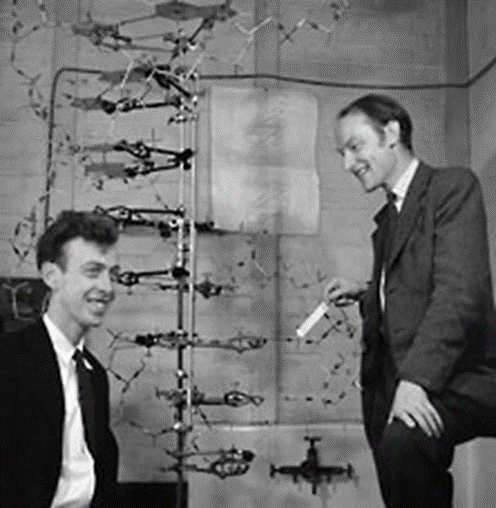
\includegraphics[width=\linewidth]{W&C,DNA双螺旋1}
		\caption{Waston和Crick发现了DNA双螺旋结构}
	\end{subfigure}
	\hfill
	\begin{subfigure}{0.3\textwidth}
		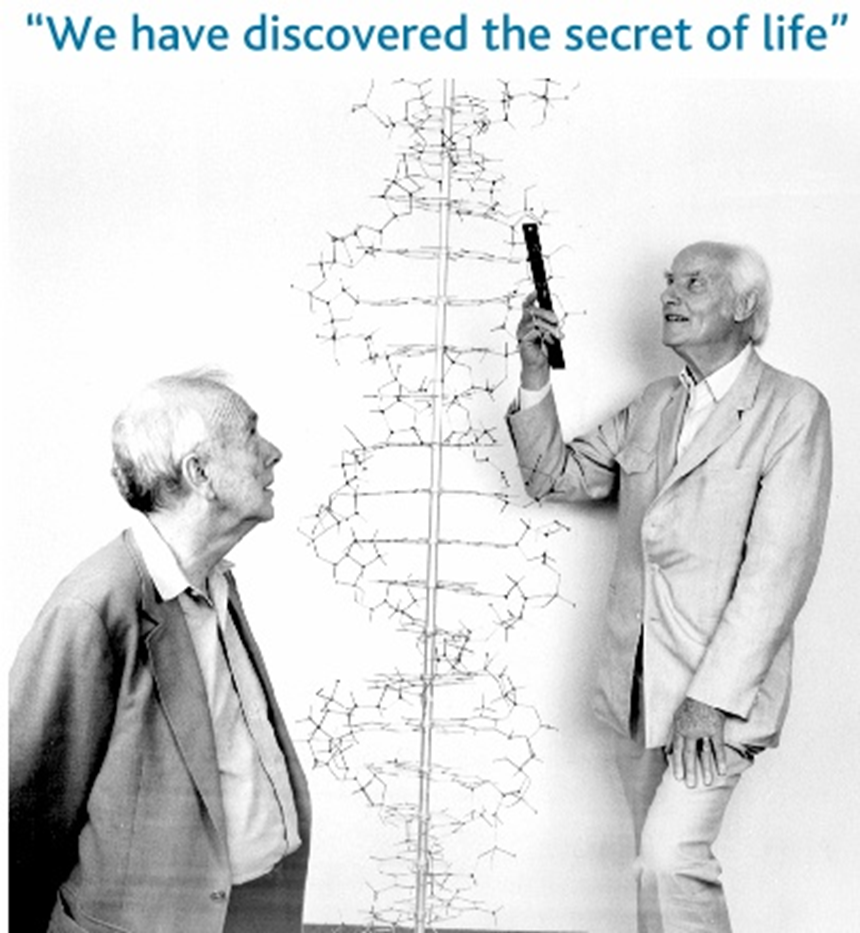
\includegraphics[width=\linewidth]{W&C,DNA双螺旋2}
		\caption{已步入古稀之年的Watson(左)和Crick(右)在讨论DNA双螺旋结构模型}
	\end{subfigure}
	\hfill
	\begin{subfigure}{0.3\textwidth}
		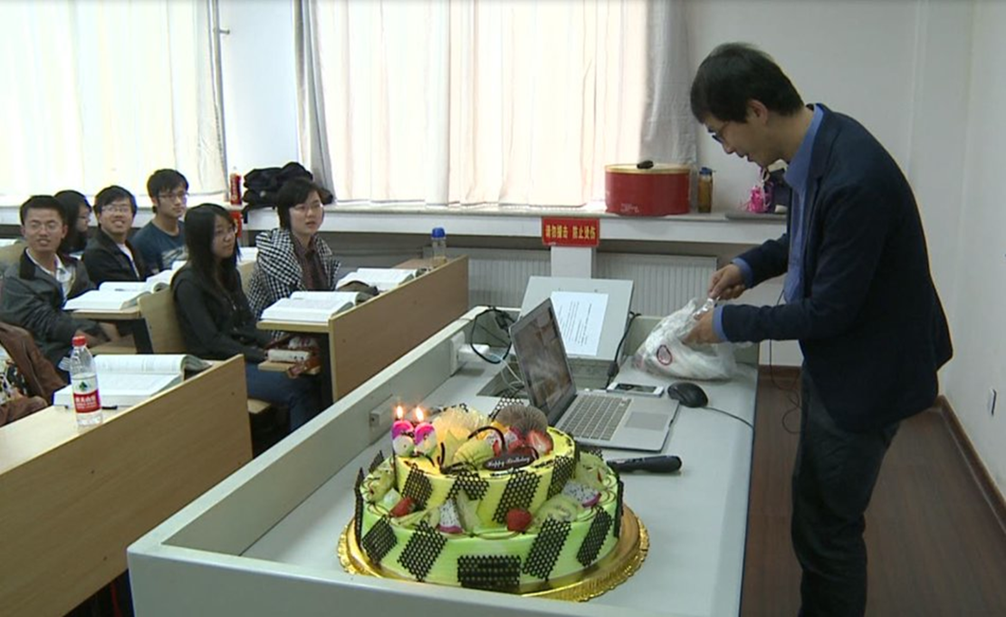
\includegraphics[width=\linewidth]{R.Young,DNA双螺旋3}
		\caption{2013年4月25日,杨荣武教授为DNA双螺旋结构庆生}
	\end{subfigure}
	\caption{DNA双螺旋结构的发现}
	\label{fig:discover_DNA_double_helix}
\end{figure}

A、B、Z螺旋的特征概括如


\paragraph{支持DNA双螺旋结构的证据}

\paragraph{DNA的非标准二级结构}

DNA可形成弯曲、十字形、三螺旋、滑移错配DNA、碱基翻转这些非标准二级结构。

形成这些结构的原因可能是受到蛋白质作用,或是DNA拥有独特的序列模体:反向重复、回文序列、镜像重复、直接重复、高嘌呤序列、高嘧啶序列(\autoref{fig:dna_specific_sequence_motif})、富含A序列、富含G序列等。

\begin{figure}[htbp]
	\centering
	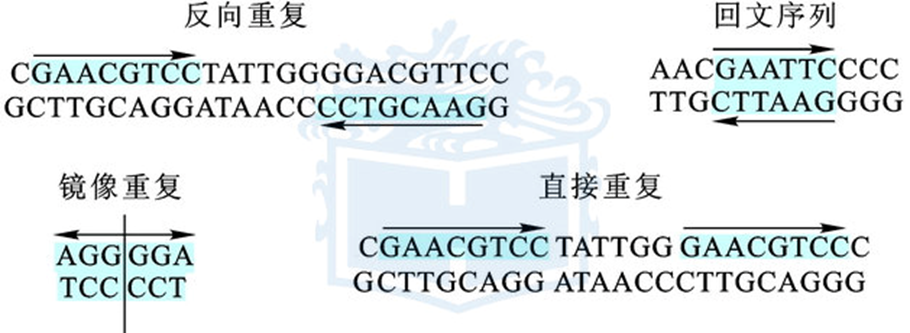
\includegraphics[width=0.7\linewidth]{Pics/DNA的特殊序列模体}
	\caption{DNA的特殊序列模体}
	\label{fig:dna_specific_sequence_motif}
\end{figure}

\begin{figure}[htbp]
	\centering
	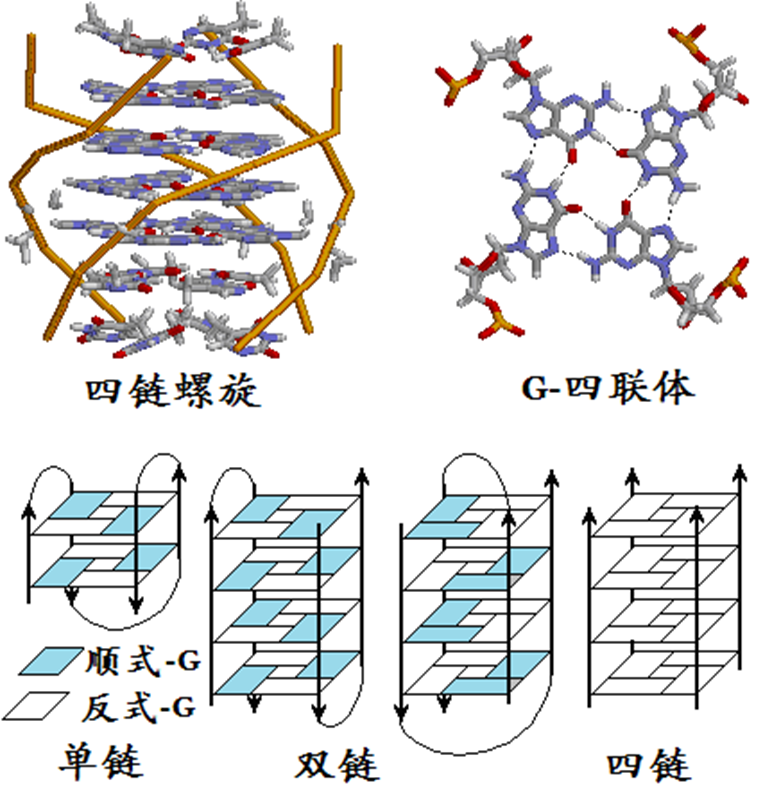
\includegraphics[width=0.5\linewidth]{Pics/DNA的四链结构}
	\caption{DNA的四链结构}
	\label{fig:dna_4strand}
\end{figure}


\subparagraph{弯曲}
\subsubsection{RNA的二级结构}

RNA有很丰富的二级结构。(\autoref{fig:rna_second_structure})自然界的RNA多数都是单链,但依然可以通过自我折叠形成局部的A型双螺旋。

\begin{figure}[htbp]
	\centering
	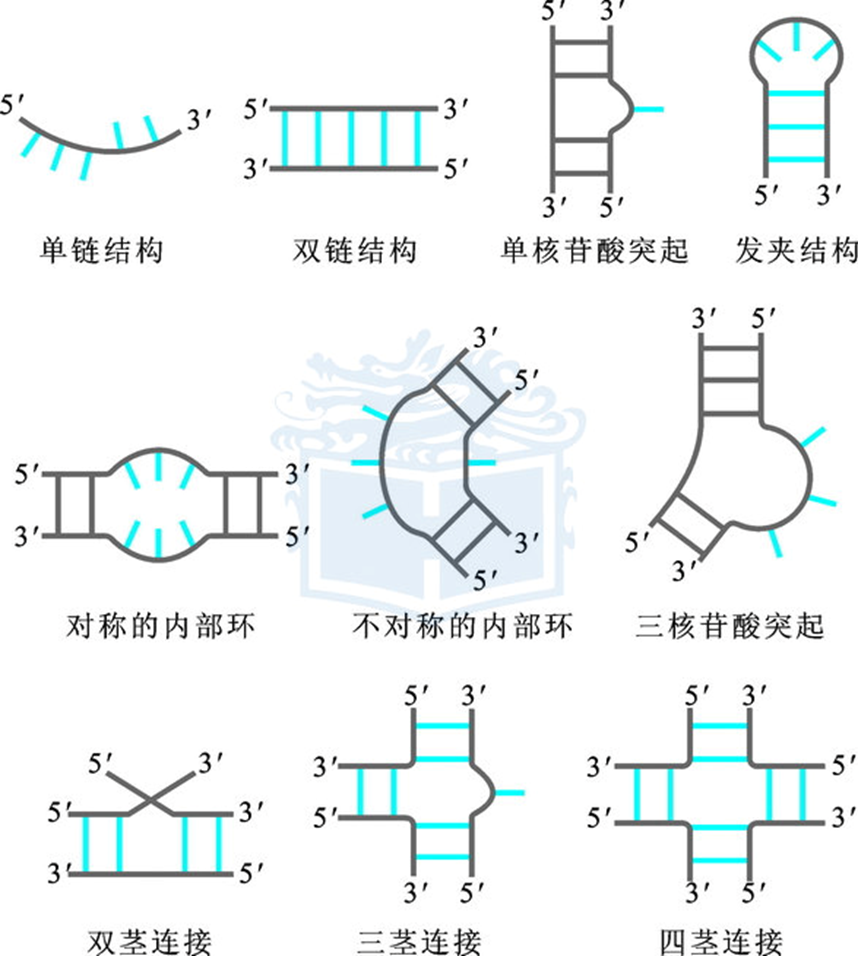
\includegraphics[width=0.7\linewidth]{Pics/RNA的二级结构}
	\caption{RNA的二级结构}
	\label{fig:rna_second_structure}
\end{figure}


\section{核酸的理化性质}

\subsubsection{紫外吸收}

\subsubsection{酸碱解离}

\subsubsection{黏度}

\subsubsection{沉淀}

\subsubsection{变性}

核酸变性不涉及任何共价键断裂,只是二级结构、三级结构的改变。

\section{酶学概论}

\subsection{酶的化学本质}

大多数酶都是蛋白质,少数酶是RNA。这种具有催化活性的RNA称为\sy{核酶}。

酶可按化学组成分类:(\autoref{fig:class_enzyme})

\begin{figure}[htbp]
	\centering
	\begin{forest}
		forest scheme
		[酶
			[单纯酶]
			[缀合酶
				[多肽链]
				[非氨基酸的辅因子
					[辅酶:结合松散,如辅酶I、辅酶II]
					[辅基:结合紧密,如FAD]
					[金属离子]]]]
	\end{forest}
	\caption{酶按化学组成的分类}
	\label{fig:class_enzyme}
\end{figure}

丧失辅因子的酶成为脱辅酶,结合了辅因子的酶称全酶。含紧密结合的金属离子的酶通常称为金属酶。

大多数核酶都含有金属离子和(或)蛋白质,仅有少数是单独的RNA。

\subsection{酶的催化性质}

酶的催化性质有:
\begin{enumerate}
	\item 高效性;
	\item 酶在活性中心与底物结合;
	\item 高度专一性;
	\item 反应条件温和;
	\item 对反应条件敏感,易失活;
	\item 受到调控;
	\item 许多酶的活性需要辅因子存在。
\end{enumerate}

下面对上述部分名词作解释。

\subsubsection{活性中心}

活性中心是酶与底物结合,直接参与催化的部位。缀合酶的活性中心还包括和底物结合的部分。多功能酶有多个活性中心。

活性中心由结合基团和催化基团构成,前者决定专一性,后者决定催化能力。但有些基团可能同时承担二者功能。

活性中心的一般特征:
\begin{description}
	\item[是三维实体,相关氨基酸残基一级结构不相邻。] 活性中心的三维实体结构是蛋白质正确折叠后的必然产物。
	\item[所占体积小] 酶上的大多数氨基酸残基并不与底物接触,起到稳定活性中心的作用。
	\item[呈裂隙、口袋状] 活性中心内部多为疏水氨基酸残基,也有少量亲水的。
	\item[只有亲水氨基酸残基可催化反应] 疏水氨基酸侧链是惰性的,无法催化反应。活性中心中出现的亲水氨基酸频次:H>C>D>R>E。
	\item[大多靠多重次级键与底物结合] 在共价催化中,酶与底物形成暂时的共价键。
	\item[结构互补性] 活性中心与底物过渡态的互补性优于底物。
	\item[具有柔性] 构象会发生改变。
\end{description}

\subsubsection{专一性}

专一性的类型:
\begin{description}
	\item[绝对专一性] 酶仅严格催化一个反应。
	\item[相对专一性] 这是大多数酶的专一性类型。包括基团专一性和键专一性。这就是说酶只作用于特定的基团或化学键。
	\item[立体专一性] 酶对具有立体异构体的底物,只作用于其中一种。进一步分为旋光异构专一性和几何异构专一性。前者即底物的D、L型,后者即底物的顺、反式。
\end{description}

酶的立体专一性还表现在能区分假手性C上两个我们看似相同的基团。例如:
\begin{itemize}
	\item 一端由\ce{C^{14}}标记的甘油,由甘油激酶催化加磷酸,只生成1-磷酸甘油。(\autoref{fig:stereospec_glycerolkinase})

	\begin{figure}[htbp]
		\centering
		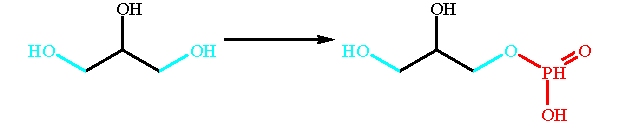
\includegraphics{甘油激酶的立体专一性}
		\caption{甘油激酶的立体专一性}
		\label{fig:stereospec_glycerolkinase}
	\end{figure}

	\item 顺乌头酸酶只会把羟基给来自草酰乙酸的\ce{-CH2-COOH},而不会给来自乙酰CoA的。(\autoref{fig:FumaraseStereoSpecificity})

	\begin{figure}[htbp]
		\centering
		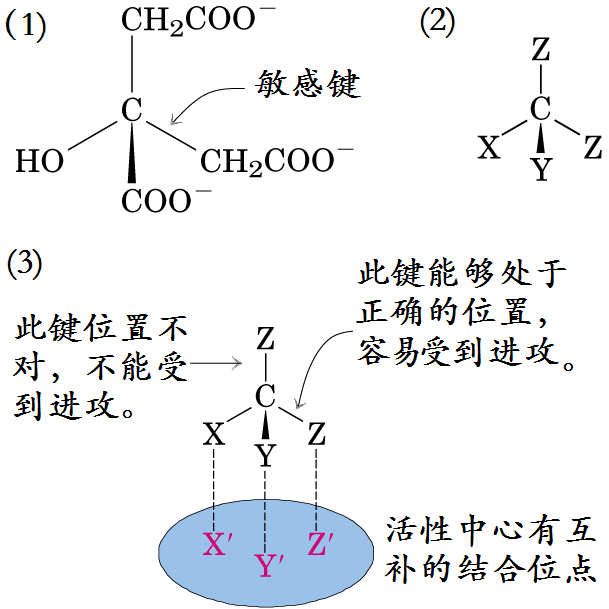
\includegraphics[width=0.3\linewidth]{Pics/顺乌头酸酶的立体专一性}
		\caption{顺乌头酸酶的立体专一性}
		\label{fig:FumaraseStereoSpecificity}
	\end{figure}

	\item 酵母乙醇脱氢酶(YADH)在催化时,辅酶NADH上的烟酰胺环,只有一侧是可以加氢或脱氢的。(\autoref{fig:yadh})

	\begin{figure}[htbp]
		\centering
		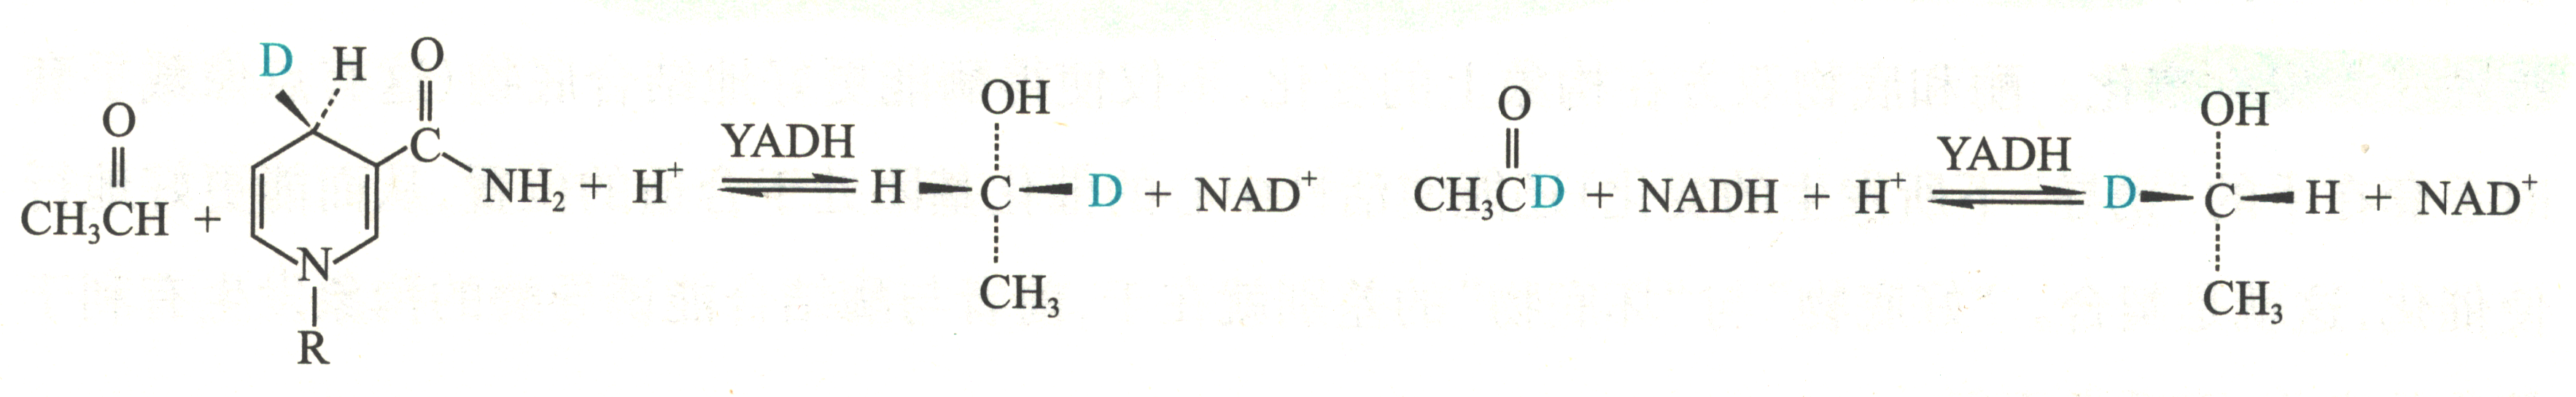
\includegraphics{YADH的立体专一性}
		\caption{YADH的立体专一性}
		\label{fig:yadh}
	\end{figure}

\end{itemize}

YADH这种专一性定为A型,有相同专一性的脱氢酶被称为A型脱氢酶,如苹果酸脱氢酶、异柠檬酸脱氢酶、乳酸脱氢酶。不具有这种专一性的酶称为B型酶,如谷氨酸脱氢酶、3-磷酸甘油脱氢酶。

有三个作用可解释酶的立体专一性:
\begin{description}
	\item[“锁与钥匙”模型] 比较过时,早已被淘汰。
	\item[“诱导契合”模型] 酶活性中心是柔性可变的。一开始酶和底物并不契合,当二者靠近,酶活性中心和底物的构象都发生变化(诱导),使活性中心更好结合底物(契合)。
	\item[“三点附着”模型] 底物在活性中心有3个结合位点,只有当3个结合位点都匹配,才会催化反应。这可以解释立体专一性。
\end{description}

\subsection{酶的分类}

根据反应的性质,把酶分为七类:(\autoref{tab:酶的分类})

\begin{table}[htbp]
	\zihao{5}
	\centering
	\begin{tabularx}{\textwidth}{|cCc|}
		\hline
		\multicolumn{1}{|c|}{类别} & \multicolumn{1}{c|}{反应性质} & 实例 \\ \hline
		\multicolumn{1}{|c|}{氧化还原酶} & \multicolumn{1}{c|}{电子转移} & 乙醇脱氢酶 \\ \hline
		\multicolumn{3}{|l|}{包括:脱氢酶,氧化酶,还原酶,过氧化物酶,过氧化氢酶,加氧酶,羟化酶} \\ \hline
		\multicolumn{1}{|c|}{转移酶} & \multicolumn{1}{c|}{分子间基团转移} & 蛋白激酶 A \\ \hline
		\multicolumn{3}{|l|}{包括:转醛酶和转酮酶,脂酰基、甲基、糖基和磷酸基转移酶,激酶,磷酸变位酶} \\ \hline
		\multicolumn{1}{|c|}{水解酶} & \multicolumn{1}{c|}{通过加水导致键的断裂} & 脂肪酶 \\ \hline
		\multicolumn{3}{|l|}{包括:酯酶,糖苷酶,肽酶,磷酸酶,硫酯酶,磷脂酶,酰胺酶,脱氨酶和核酸酶} \\ \hline
		\multicolumn{1}{|c|}{裂合酶} & \multicolumn{1}{c|}{消除反应,产生双键} & 碳酸酐酶 \\ \hline
		\multicolumn{3}{|l|}{包括:脱羧酶,醛缩酶,水合酶,脱水合酶,合酶,裂解酶} \\ \hline
		\multicolumn{1}{|c|}{异构酶} & \multicolumn{1}{c|}{分子内的重排} & TIM \\ \hline
		\multicolumn{3}{|l|}{包括:消旋酶,差向异构酶,异构酶,变位酶} \\ \hline
		\multicolumn{1}{|c|}{连接酶} & \multicolumn{1}{c|}{水解 ATP 与分子之间的连接偶联} & DNA 连接酶 \\ \hline
		\multicolumn{3}{|l|}{包括:合成酶和羧化酶} \\ \hline
		\multicolumn{1}{|c|}{转位酶} & \multicolumn{1}{c|}{与NTP水解或氧化还原酶反应偶联的物质跨膜转运或在膜内的分离} &  \\ \hline
		\multicolumn{3}{|l|}{包括:F型质子泵、ABC超家族等} \\ \hline
	\end{tabularx}
	\caption{酶的分类}
	\label{tab:酶的分类}
\end{table}

\begin{tx}[:区分合酶和合成酶]

	合酶催化的反应是缩合反应,但并没有与ATP的水解相偶联,而合成酶属于第六类酶,所催化的反应一定与ATP或者它的等价物的降解相偶联。
\end{tx}

\begin{qj}[:七大类酶]
	想要记住七大类酶的名称和顺序,记住前六类分别是:养(氧化还原酶)鱼(转移酶)水(水解酶)活(裂合酶)鱼(异构酶)活(合成酶),再加上第七类转位酶即可。
\end{qj}



\section{酶动力学}

\subsection{影响酶促反应速率的因素}

\subsubsection{外因}

\paragraph{温度}

温度对酶促反应速率的关系图象呈倒V型,最大值处为酶的最适温度。温度系数(即范特霍夫系数)Q$_{10}$表示温度每上升\SI{10}{\celsius},反应速率加快的倍数。

偏离最适温度,高温使酶变性,低温不变性,但活性也降低。

酶的最适温度不是酶的特征性常数,还与反应持续时间有关。如有的酶只能短时间耐受高温。

\paragraph{pH}



\subsubsection{内因}

内因就是酶浓度和底物浓度。

\begin{description}
	\item[酶浓度] 底物过量时,反应速率与酶浓度成正比。
	\item[底物浓度] 酶的浓度一定时,反应速率与底物的关系呈双曲线或S型,且具有饱和动力学特征(存在最大速率)。这一饱和动力学特征可用“酶-底物中间物”假说来解释:
	\begin{center}
		E+S$\longrightarrow$ES$\longrightarrow$EP$\longrightarrow$E+P
	\end{center}
\end{description}

\subsection{米氏动力学}

\subsubsection{米氏方程}

米氏方程基于下面三个条件:
\begin{itemize}
	\item 反应速率为初速率;
	\item [ES]不变;
	\item 反应速率与底物浓度成正比(质量作用定律)。
\end{itemize}

米氏方程可写成:
\[v=\frac{v_{\text{max}}[\text{S}]}{[\text{S}]+K_{\text{m}}}\]
其中:
\begin{itemize}
	\item $v$:反应初速率,因变量;
	\item $V_{\text{max}}$:反应的最大速率,为常数;
	\item $[\text{S}]$:底物浓度,自变量;
	\item $K_{\text{m}}$:米氏常数。
\end{itemize}

\subsubsection{米氏方程的解读}

解读可从四个与酶自身有关的常数入手,两个在米氏方程内:$K_{\text{m}}$和$V_{\text{max}}$;两个在米氏方程外:$k_{\text{cat}}$和$\displaystyle\frac{k_{\text{cat}}}{K_{\text{m}}}$。

\paragraph{$K_{\text{m}}$}

\begin{itemize}
	\item 反应对酶对底物的亲和力,$K_{\text{m}}$越大,酶对底物的亲和力越低;
	\item $K_{\text{m}}$是反应初速率为$\displaystyle\frac{1}{2} V_{\text{max}}$时的底物浓度;
\end{itemize}

\paragraph{$V_{\text{max}}$}

一个酶促反应的$V_{\text{max}}$与酶的浓度有关。$V_{\text{max}}$从来不能被直接测定到。

\paragraph{$k_{\text{cat}}$}

$k_{\text{cat}}$指的是单位时间内,酶能把多少分子的底物转换为产物,称为酶的周转数。

对于米氏酶,$\displaystyle k_{\text{cat}}=\frac{V_{\text{max}}}{[E_{\text{t}}]}$。

\paragraph{$k_{\frac{\text{cat}}{K_{\text{m}}}}$}

$\frac{k_{\text{cat}}}{K_{\text{m}}}$是一个表观二级速率常数。

可通过$\frac{k_{\text{cat}}}{K_{\text{m}}}$直接比较不同酶对底物的催化效率,从进化上衡量一个酶的完美程度。当一个酶极其完美时,$\frac{k_{\text{cat}}}{K_{\text{m}}}$就完全由物理扩散定律限制。磷酸丙糖异构酶(TIM)是公认最完美的酶,即“酶神”。

\subsubsection{米氏方程的双重性}

如所示:

\begin{figure}[htbp]
	\centering
	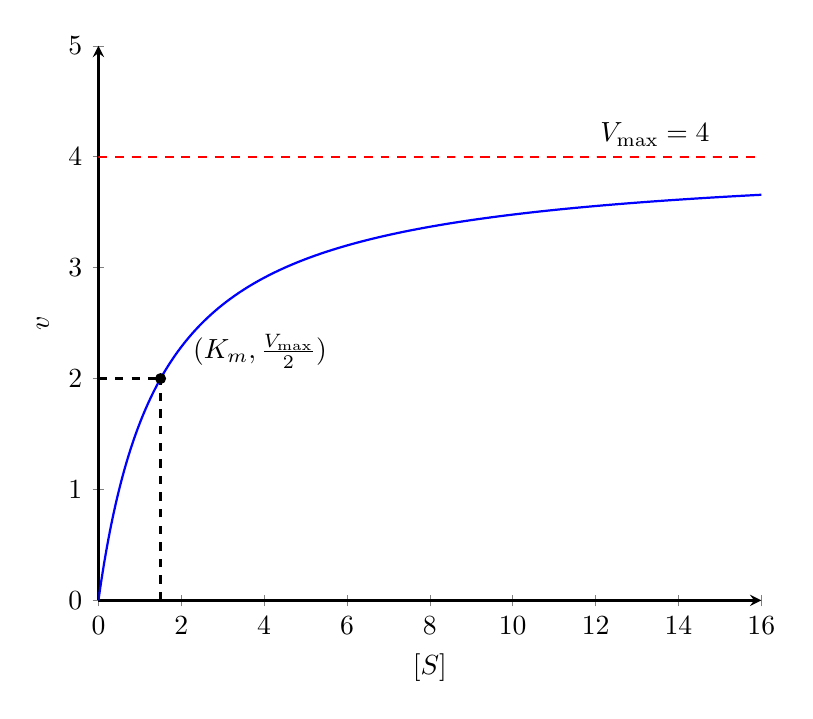
\begin{tikzpicture}
	\begin{axis}[
		xlabel={$[\text{S}]$},
		ylabel={$v$},
		xmin=0, xmax=16,      % 将xmax稍增大到16以容纳标注
		ymin=0, ymax=5,
		grid=none,
		samples=1000,
		axis lines=left,
		thick,
		smooth,
		width=10cm,           % 调整图像宽度以提供更多空间
		]
		\addplot[blue, domain=0:16] {(4*x)/(1.5 + x)};
		\addplot[dashed, red, domain=0:16] {4};

		% 调整标注位置与对齐方式
		\node[left] at (axis cs:15,4.2) {$V_{\max} = 4$}; % 左对齐避免超出右边界

		\draw[dashed] (axis cs:1.5,0) -- (axis cs:1.5,2);
		\draw[dashed] (axis cs:0,2) -- (axis cs:1.5,2);
		\fill (axis cs:1.5,2) circle (2pt)
		node[above right, xshift=8pt] {$(K_m, \frac{V_{\max}}{2})$}; % 右上方标注避免超出左边界
	\end{axis}
	\end{tikzpicture}
	\caption{米氏方程的曲线}
\end{figure}
\begin{itemize}
	\item $[\text{S}]\ll K_{\text{m}}$时,反应速率与底物浓度成正比,符合一级动力学;
	\item $[\text{S}]\gg K_{\text{m}}$时,反应速率接近$V_{\text{max}}$,即使增加底物浓度,反应速率也几乎不增加,符合零级动力学。
\end{itemize}

\subsubsection{米氏方程的线性转换}

线性转换的优势是便于减小误差对作图的干扰。下面介绍几种常见的线性转换方法。

\paragraph{Lineweaver-Burk双倒数作图}

将米氏方程两边取倒数可得:

\[\frac{1}{v} = \frac{K_\text{m}}{v_{\text{max}}} \cdot \frac{1}{[\text{S}]} + \frac{1}{v_{\text{max}}}\]

转换以后,以$\dfrac{1}{[\text{S}]}$为横轴、$\dfrac{1}{v}$为纵轴作图,便可得到线性图像。(\autoref{fig:双倒数法作图})

\begin{figure}[htbp]
	\centering
	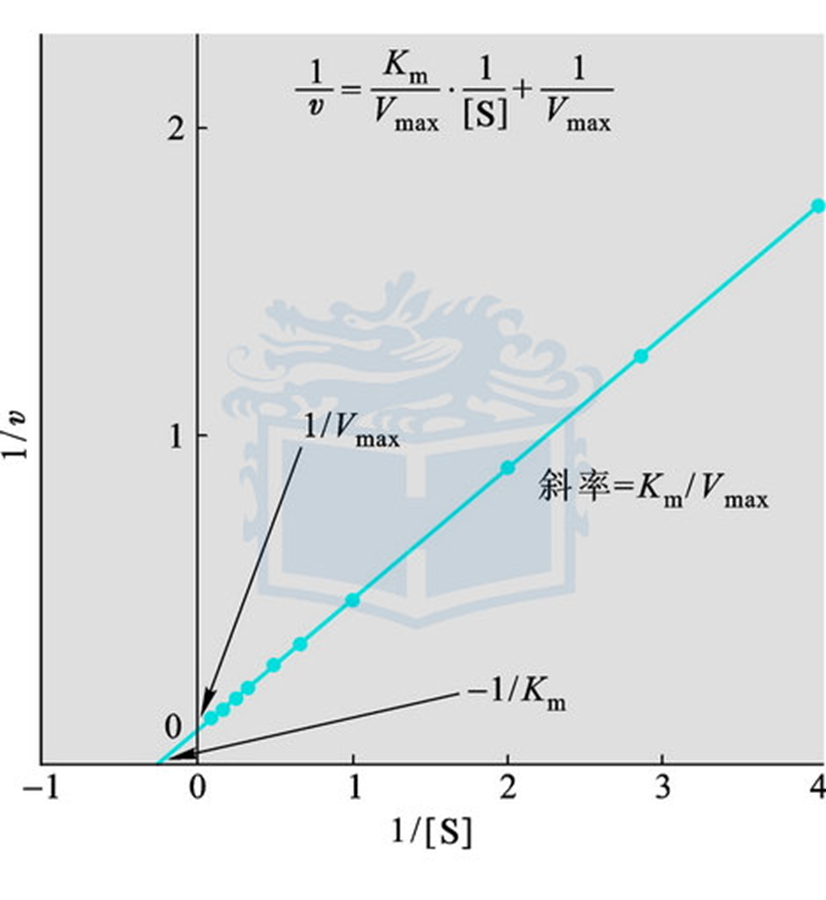
\includegraphics[width=0.7\linewidth]{Pics/双倒数法作图}
	\caption{双倒数法作图}
	\label{fig:双倒数法作图}
\end{figure}

其中:

\begin{itemize}
	\item 纵截距:$\dfrac{1}{V_{\text{max}}}$;
	\item 横截距:$-\dfrac{1}{K_{\text{m}}}$;
	\item 斜率:$\dfrac{K_{\text{m}}}{v_{\text{max}}}$。
\end{itemize}

缺陷:双倒数法作图会扩大误差。

\paragraph{Eadie-Hofstee作图}

\[v = -K_{\text{m}} \frac{v}{[\text{S}]} + v_{\text{max}}\]

以$\dfrac{v}{[\text{S}]}$为横轴、$v$为纵轴作图,其中:(\autoref{fig:eadie-hofstee})

\begin{figure}[htbp]
	\centering
	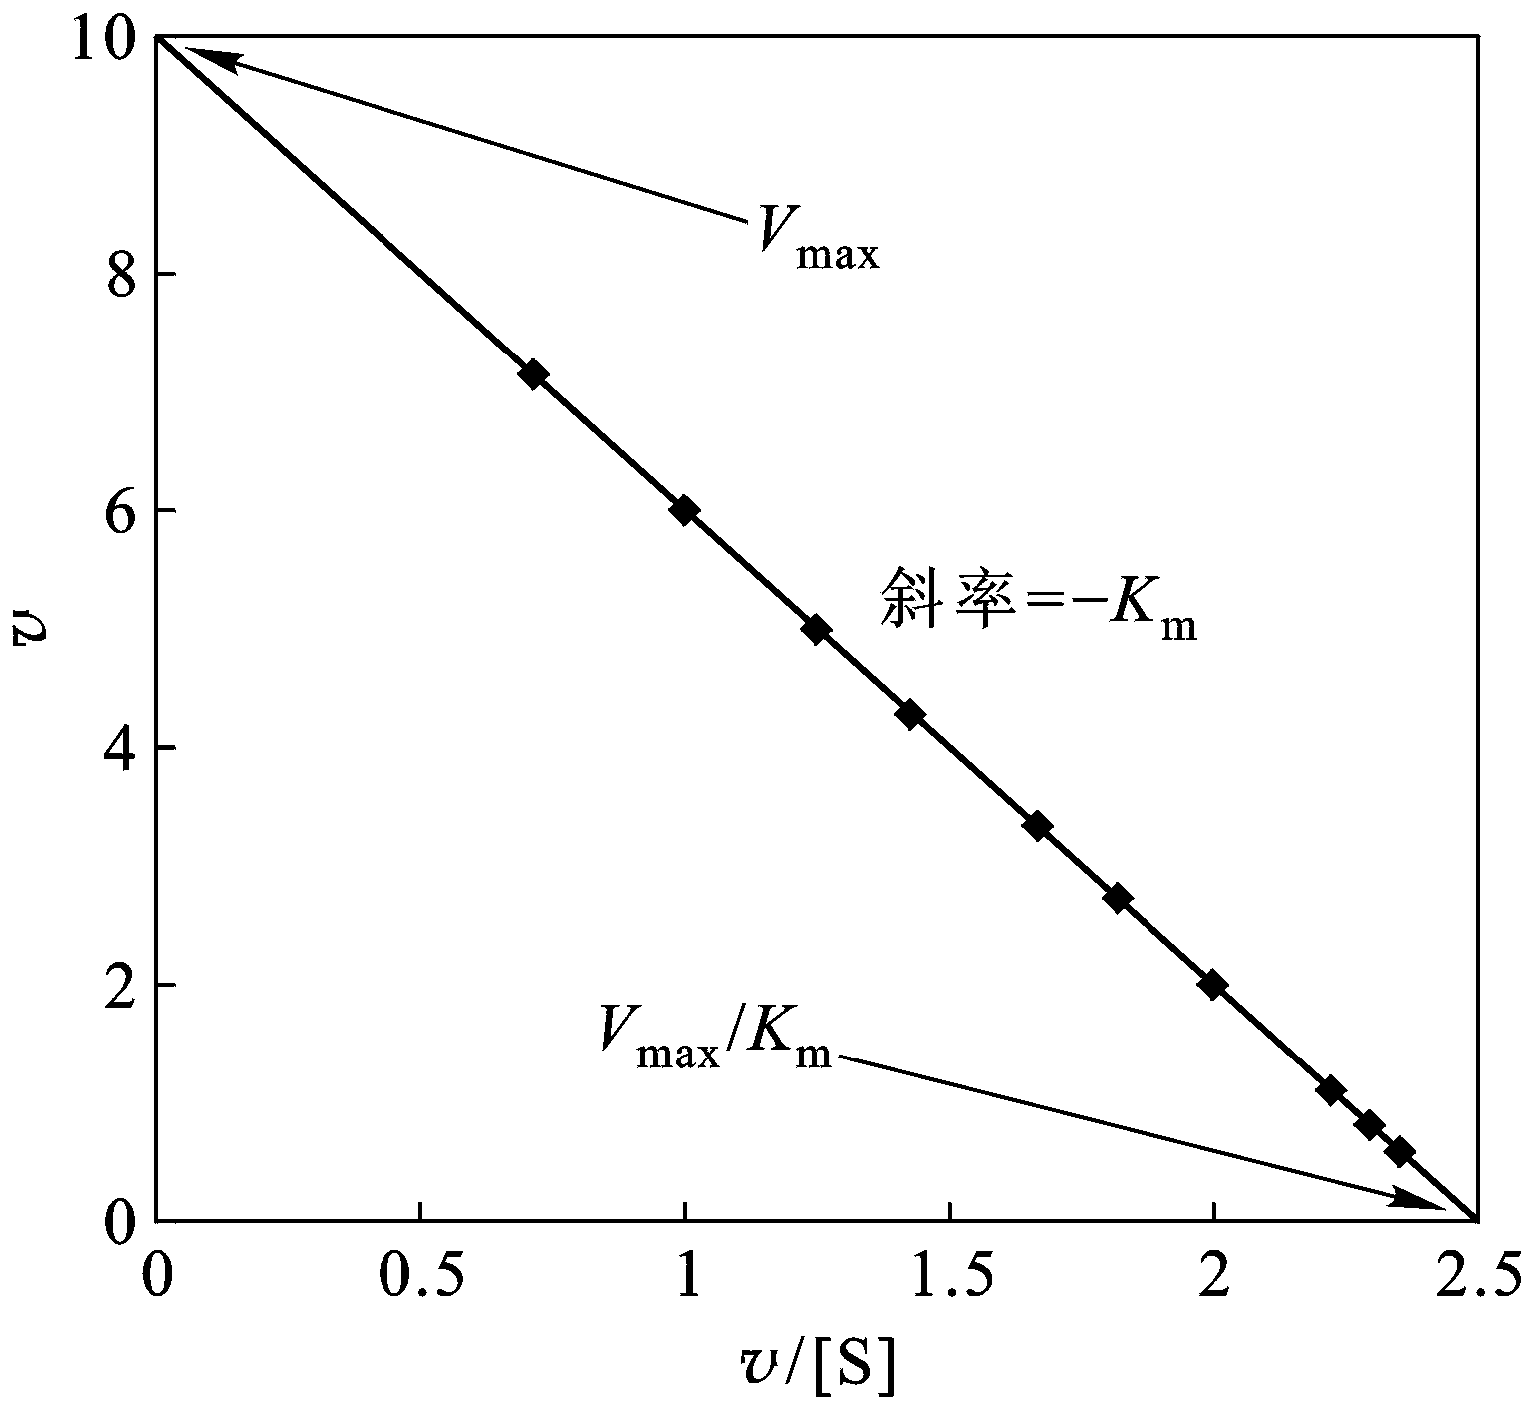
\includegraphics[width=0.5\linewidth]{Pics/Eadie-Hofstee作图}
	\caption{Eadie-Hofstee作图}
	\label{fig:eadie-hofstee}
\end{figure}

\begin{itemize}
	\item 纵截距:$v_{\text{max}}$;
	\item 横截距:$\dfrac{v_{\text{max}}}{K_{\text{m}}}$;
	\item 斜率:$-K_{\text{m}}$。
\end{itemize}

缺陷:同样会扩大误差,但没有双倒数法严重;$v$的误差会同时影响两个轴。

\paragraph{Hanes-Wolff作图}

\[\frac{[\text{S}]}{v} = \frac{1}{v_{\text{max}}} \cdot [\text{S}] + \frac{K_{\text{m}}}{v_{\text{max}}}\]

以$[\text{S}]$为横轴、$\dfrac{[\text{S}]}{v}$为纵轴作图,其中:(\autoref{fig:hanes-wolff})

\begin{figure}[htbp]
	\centering
	\includegraphics[width=0.5\linewidth]{"Pics/Hanes-Wolff 作图"}
	\caption{Hanes-Wolff作图}
	\label{fig:hanes-wolff}
\end{figure}

\begin{itemize}
	\item 纵截距:$\dfrac{K_{\text{m}}}{v_{\text{max}}}$;
	\item 横截距:$-K_{\text{m}}$;
	\item 斜率:$\dfrac{1}{v_{\text{max}}}$。
\end{itemize}

\paragraph{直接线性化作图}

\[v_{\text{max}} = \frac{v}{[\text{S}]} \cdot K_{\text{m}} + v\]

在直接线性化作图中,以$K_{\text{m}}$为横轴、$v_{\text{max}}$为纵轴,可以作出无数条直线。它们的交点坐标就是$(K_{\text{m}},V_{\text{max}})$。(\autoref{fig:直接线性化作图})

\begin{figure}[htbp]
	\centering
	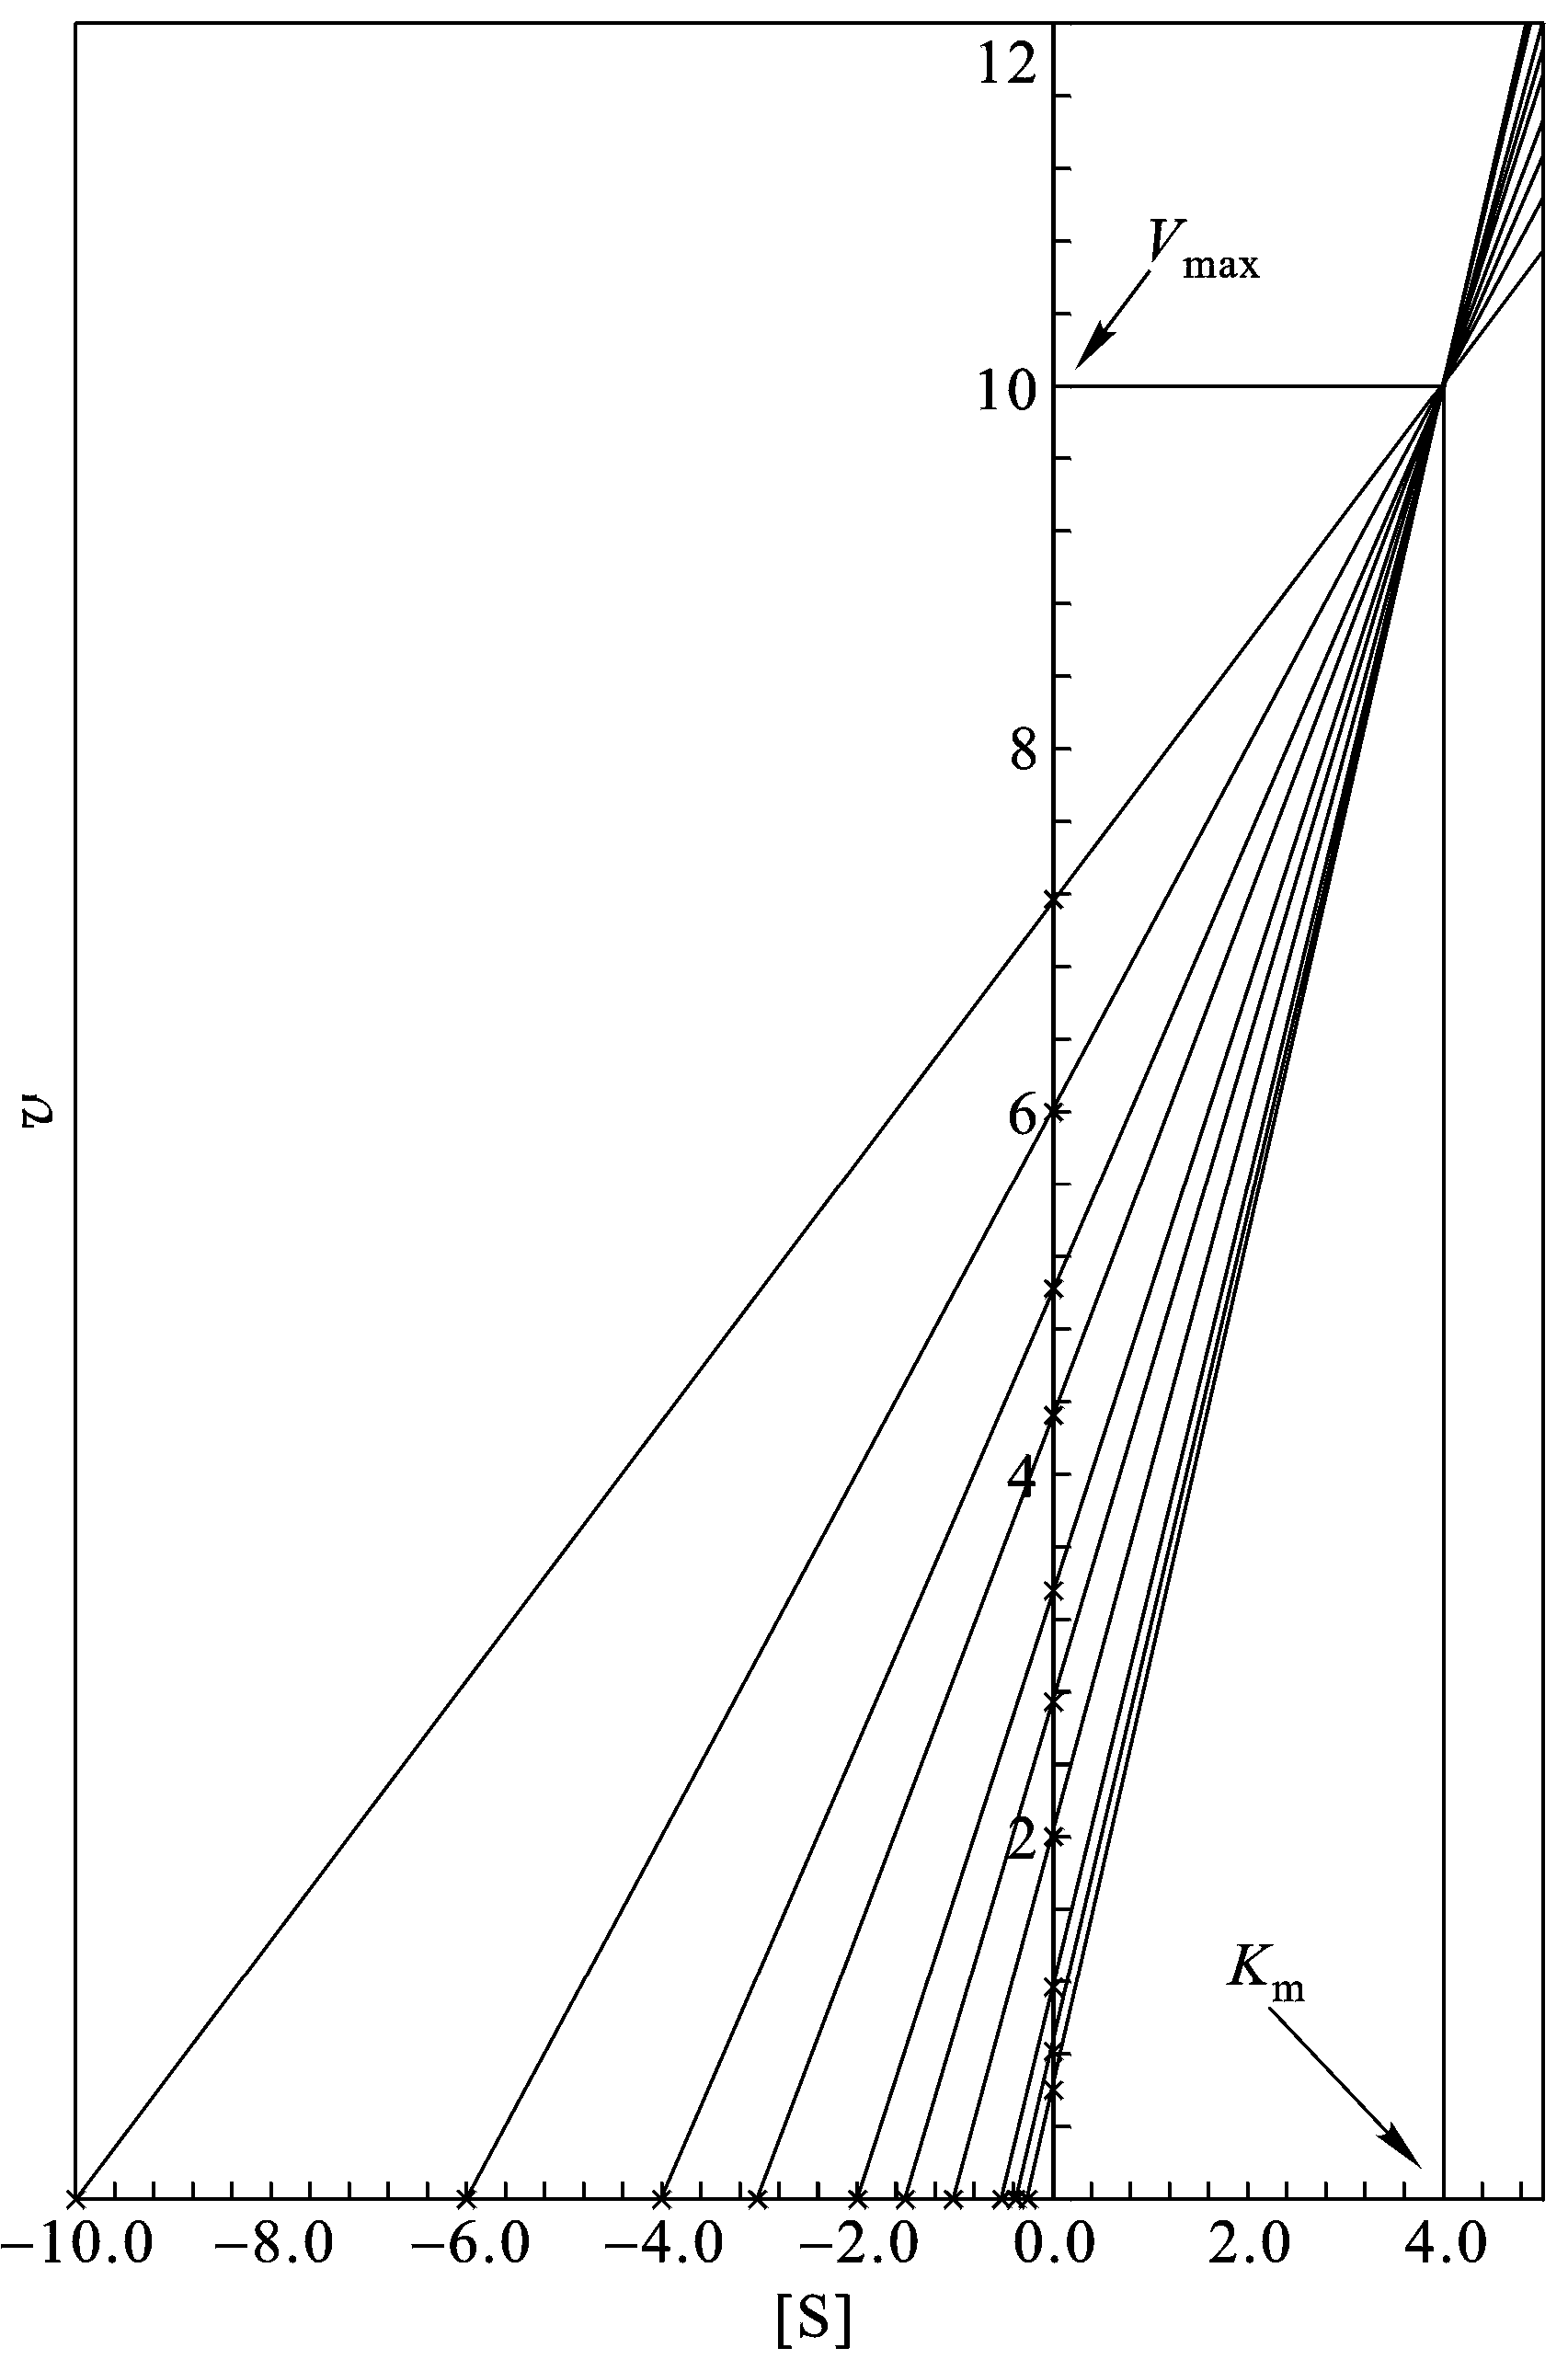
\includegraphics[width=0.5\linewidth]{直接线性化作图}
	\caption{直接线性化作图}
	\label{fig:直接线性化作图}
\end{figure}

\subsection{米氏酶抑制剂动力学}

酶的抑制剂分为可逆性抑制剂和不可逆性抑制剂两类(\autoref{fig:米氏酶抑制剂的分类})。不可逆抑制剂的作用有时间依赖性。

\begin{figure}[htbp]
	\centering
	\begin{forest}
		forest scheme
		[抑制剂
			[可逆性抑制剂
				[竞争性抑制剂]
				[非竞争性抑制剂]
				[反竞争性抑制剂]]
			[不可逆性抑制剂
				[基团特异性抑制剂]
				[底物类似物抑制剂]
				[过渡态类似物抑制剂]
				[自杀型抑制剂]]]
	\end{forest}
	\caption{米氏酶抑制剂的分类}
	\label{fig:米氏酶抑制剂的分类}
\end{figure}

\subsubsection{可逆性抑制剂}

在下面叙述中,定义:$\alpha=1+\dfrac{[\text{I}]}{K_{\text{I}}}$

三种可逆性抑制剂对酶的影响见\autoref{tab:三种可逆性抑制剂对酶的影响}。

\begin{table}[htbp]
	\centering
	\begin{tabularx}{\textwidth}{|c|C|C|C|}
		\hline
		\textbf{抑制剂类型} & \textbf{$K_{\text{m}}$} & \textbf{$V_{\text{max}}$} & \textbf{米氏方程} \\ \hline
		竞争性抑制剂 & 增加 & 不变 & $v = \frac{V_{\text{max}} [S]}{\alpha K_{\text{m}} + [S]}$ \\ \hline
		非竞争性抑制剂 & 不变 & 减少 & $v = \frac{V_{\text{max}} [S]}{(K_{\text{m}} + [S])\alpha}$ \\ \hline
		混合型抑制剂 & 增加 & 减少 & --- \\ \hline
		反竞争性抑制剂 & 减少 & 减少 & $v = \frac{V_{\text{max}} [S]}{K_{\text{m}} + [S]\alpha}$ \\ \hline
	\end{tabularx}
	\caption{三种可逆性抑制剂对酶的影响}
	\label{tab:三种可逆性抑制剂对酶的影响}
\end{table}

世上没有完全单纯的非竞争性抑制剂,而混合型抑制剂指的就是兼具非竞争性抑制剂和竞争性抑制剂特性的抑制剂。

\subsubsection{不可逆性抑制剂}

\subsection{别构酶的动力学}



\section[激素和信号转导]{激素及其受体介导的信号转导}

\subsection{激素的一般性质}

\subsubsection{激素的定义}

激素是一类非营养的、微量就能起作用的、在细胞之间传递信息的物质。它最显著的特征就是含量低。

分泌激素的细胞称内分泌细胞,受激素作用的细胞称靶细胞。根据作用的距离,把激素分为内分泌激素、神经内分泌激素、旁分泌激素、自分泌激素、内部分泌激素(\autoref{fig:hormone_types}、\autoref{tab:hormone_types})。

\begin{figure}[htbp]
	\centering
	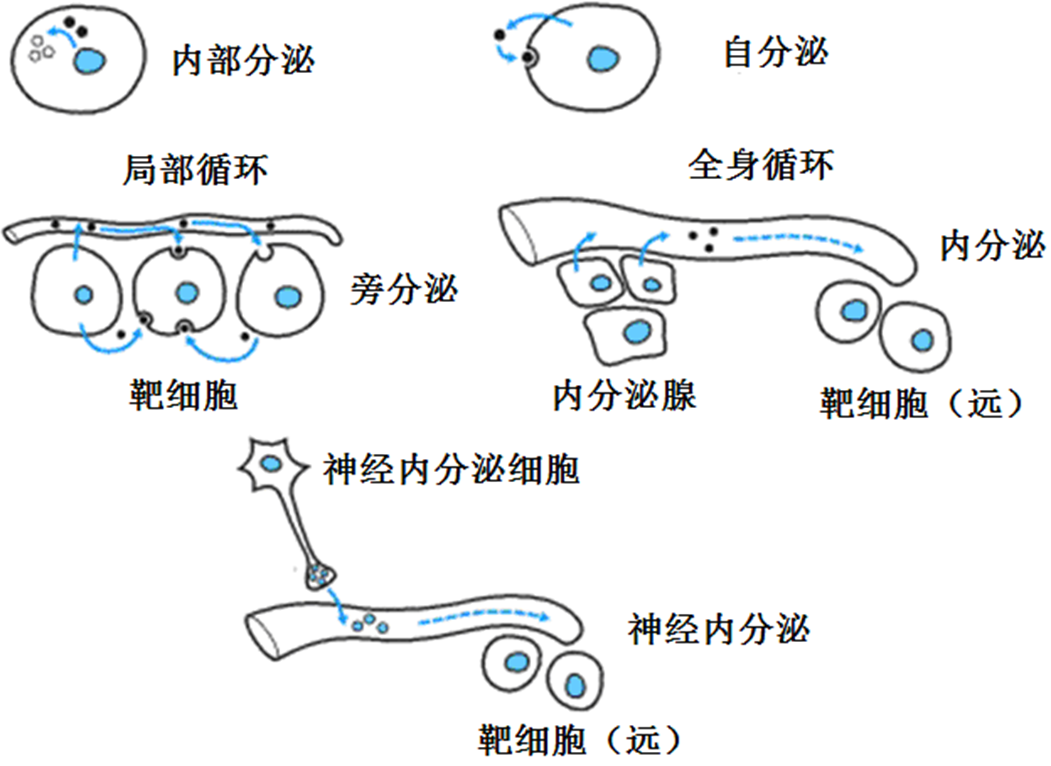
\includegraphics[width=0.7\linewidth]{Pics/激素作用类型}
	\caption{激素的5种分泌方式}
	\label{fig:hormone_types}
\end{figure}

\begin{table}[htbp]
	\centering
	\begin{tabularx}{\textwidth}{|c|X|X|}
		\hline
		\multicolumn{1}{|c|}{分泌方式} & \multicolumn{1}{c|}{作用对象} & \multicolumn{1}{c|}{举例} \\ \hline
		内分泌 & 较远的靶细胞 & 大多数激素 \\ \hline
		神经内分泌激素 & 同上,但是由特殊的神经内分泌细胞(同时也是神经细胞)分泌 & 哺乳动物下丘脑产生的激素 \\ \hline
		旁分泌激素 & 邻近的细胞 & 前列腺素、阿片肽、一些多肽生长因子 \\ \hline
		自分泌激素 & 原来分泌它的细胞 & 白介素-2、某些生长因子、某些原癌基因的产物 \\ \hline
		内部分泌激素 & 不分泌到胞外 & 胰岛素类生长因子结合蛋白3(IGFBP-3) \\ \hline
	\end{tabularx}
	\caption{激素的5种作用方式}
	\label{tab:hormone_types}
\end{table}

按照更广泛的激素的定义,生长因子、细胞因子和神经递质等细胞间信号分子也属于激素。

\subsubsection{激素的化学本质、分类}

按照来源和化学本质,把激素分为肽类或蛋白质激素、固醇类激素、氨基酸衍生物激素、脂肪酸衍生物激素。

\begin{itemize}
	\item 肽类或蛋白质激素种类最多,大小各异;
	\item 固醇类激素均衍生于胆固醇,包括维生素D、肾上腺皮质激素、性激素。所有固醇类激素都具有相同的环结构,但是空间取向不同,这就决定了激素作用的特异性;
	\item 氨基酸衍生物激素的前体是氨基酸,如Tyr、Trp;
		\begin{itemize}
			\item 衍生于Tyr的激素有:肾上腺素、去甲肾上腺素、甲状腺素;
			\item 衍生于Trp的激素有:5-羟色胺、褪黑素。
		\end{itemize}
	\item 脂肪酸衍生物激素衍生于脂肪酸,如花生四烯酸。这些激素包括:前列腺素、凝血恶烷、白三烯等。
\end{itemize}

按照溶解性质,激素可分为水溶性激素和脂溶性激素(\autoref{tab:hormone_differ})。

\begin{table}[h]
	\centering
	\begin{tabular}{|c|p{15em}|p{12em}|}
		\hline
		特征 & \multicolumn{1}{c|}{\makecell{脂溶性激素\\(如固醇类激素和甲状腺素)}} & \multicolumn{1}{c|}{\makecell{水溶性激素\\(如肽类激素和肾上腺素)}} \\ \hline
		合成后贮存 & 除了甲状激素以外很少见 & 是的 \\ \hline
		结合蛋白 & 总是 & 少见 \\ \hline
		半衰期 & 长(数小时或数天) & 短(几分钟) \\ \hline
		受体 & 细胞质或细胞核,极少数在细胞膜 & 总是在细胞膜 \\ \hline
		作用机制 & 直接 & 间接(通过第二信使) \\ \hline
	\end{tabular}
	\caption{脂溶性激素和水溶性激素的性质比较}
	\label{tab:hormone_differ}
\end{table}

\subsubsection{激素的生物合成}

\begin{enumerate}
	\item 肽类或蛋白质激素:绝大多数都是单一基因编码,少数是多个。

	前激素原$\xrightarrow{\text{内质网}}$激素原$\xrightarrow{\text{高尔基体}}$激素$\xrightarrow{\text{分泌小泡}}$出胞
	\item 固醇类激素合成主要发生在光面内质网,但少数反应在线粒体。
	\item 氨基酸衍生物是对氨基酸侧链修饰而成;
	\item 脂肪酸衍生物主要是花生四烯酸在特定酶催化下形成。
\end{enumerate}

\subsubsection{激素的定量}

放射免疫测定法(RIA)可以精确定量激素。

RIA的原理是同位素标记的激素(Ag*)和非同位素标记的激素(Ag)都能与特异性抗体结合,二者竞争结合位点。那么,一个只含有Ag*和Ab的体系,自然全都是Ag*-Ab复合物。当Ag加入,处于结合状态的Ag*和游离的Ag*比率$\displaystyle\frac{\text{Ag*-Ab}}{\text{Ag*}}$会下降。以$\displaystyle\frac{\text{Ag*-Ab}}{\text{Ag*}}$为纵轴、$(\text{Ag*}+\text{Ag})$为横轴作标准曲线。未知量的激素在同一体系中反应,可根据标准曲线获得激素的含量。(\autoref{fig:ria})

\begin{figure}[h]
	\centering
	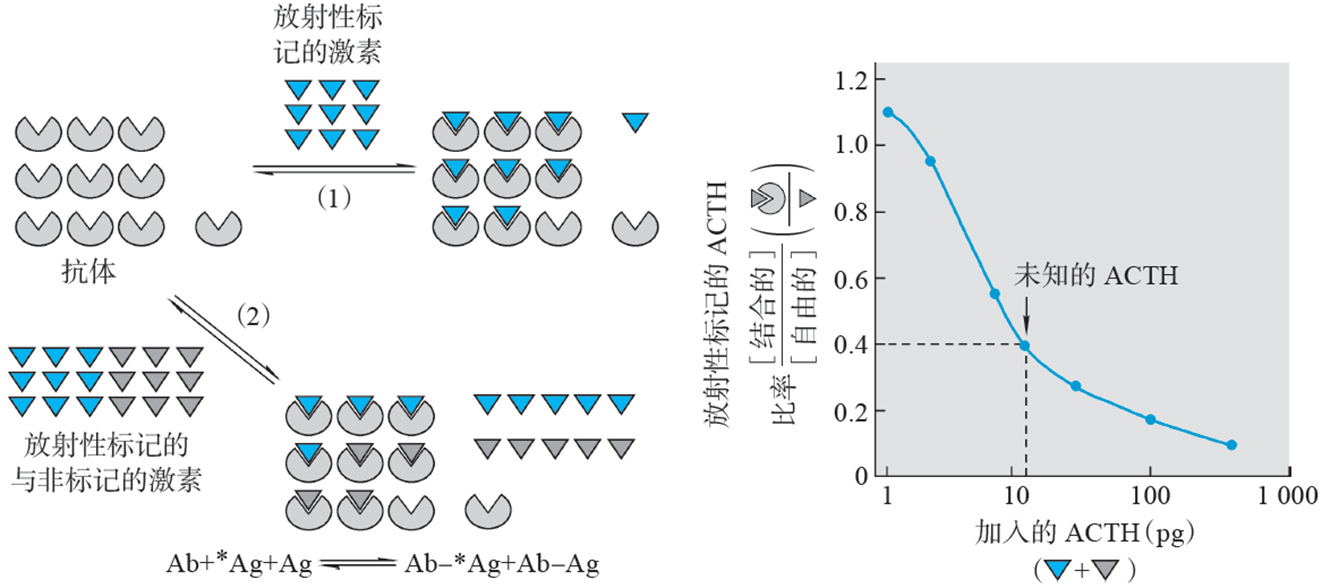
\includegraphics[width=\textwidth]{Pics/RIA}
	\caption{RIA的测定原理(以促肾上腺皮质激素ACTH为例)}
	\label{fig:ria}
\end{figure}

\subsection{激素作用的一般特征}

\subsubsection{特异性}

这是依赖于激素与特异性受体的结合实现的。

